%  author: Donny SHEN 
%  Class: MATH 2102
%  Complete Date: 2025.01.04
%  Last Modification: 2025.01.21

\documentclass[12pt]{ctexart}

% 宏包加载
\usepackage{tikz}
\usepackage{newtxtext, geometry, amsmath, amssymb}
\usepackage{amsthm}
\usepackage{xpatch}
\usepackage[strict]{changepage}
\usepackage{multicol}
\usepackage{pdfpages}
\usepackage[fontsize=14pt]{fontsize}
\usepackage{esvect}
\usepackage{xcolor} % 加载颜色宏包
\usepackage{tocloft} % 自定义目录样式
\usepackage{tcolorbox}
\usepackage{graphicx}
\usepackage{hyperref}
\hypersetup{
    colorlinks=false,  % 禁用超链接的颜色
    pdfborder={0 0 0}  % 移除超链接的边框
}

\tcbuselibrary{most}
% 加载文献引用所需宏包
\usepackage[backend=biber,style=gb7714-2015,citestyle=numeric-comp,gbalign=gb7714-2015]{biblatex}
\addbibresource{reference.bib}
\newtheorem*{lemma}{引理}
\newtheorem*{theorem}{定理}
\geometry{
    a4paper,         % 使用 A4 纸
    left=1cm,        % 左边距
    right=1cm,       % 右边距
    top=2.5cm,       % 上边距
    bottom=2.5cm     % 下边距
}

\renewcommand{\contentsname}{\hfill\centering\zihao{2} 目录\hfill~}

\begin{document}
\title{数学分析拓展3大作业} % 文档标题
\newpage
\tableofcontents % 生成目录
\newpage



\section{第一部分:作业题整理} % 无编号的 section

\setcounter{section}{1} % 手动设置章节编号为 1
\setcounter{subsection}{0} % 手动设置章节编号为 1
\subsection{周期函数的Fourier级数作业题} 
\subsubsection*{1.1.1}
\noindent 证明 $n$ 次三角多项式
\[
T_n(x) = \sum_{k=0}^n \left( a_k \cos kx + b_k \sin kx \right)
\]
的 Fourier 级数就是它自己。

\begin{proof}
在区间 $[-\pi, \pi]$ 上将三角多项式
\[
T_n(x) = \sum_{k=0}^n \left(a_k \cos kx + b_k \sin kx \right)
\]
作傅里叶级数展开,设傅里叶级数展开形式为
\[
\sum_{k=0}^n \left(a_k' \cos kx + b_k' \sin kx \right).
\]

系数 $a_n', b_n'$ 计算如下:
\[
a_0' = \frac{1}{\pi} \int_{-\pi}^\pi f(x) dx = \frac{1}{\pi} \int_{-\pi}^\pi \left[\sum_{k=0}^n \left(a_k \cos kx + b_k \sin kx \right) \right] dx = 2a_0.
\]

对任意自然数 $m$,
\[
a_m' = \frac{1}{\pi} \int_{-\pi}^\pi f(x) \cos mx \, dx = \frac{1}{\pi} \int_{-\pi}^\pi \left[\sum_{k=0}^n \left(a_k \cos kx + b_k \sin kx \right) \right] \cos mx \, dx \\ = \begin{cases} a_m, & m \leq n, \\ 0, & m > n. \end{cases}
\]

\[
b_m' = \frac{1}{\pi} \int_{-\pi}^\pi f(x) \sin mx \, dx = \frac{1}{\pi} \int_{-\pi}^\pi \left[\sum_{k=0}^n \left(a_k \cos kx + b_k \sin kx \right) \right] \sin mx \, dx \\ = \begin{cases} b_m, & m \leq n, \\ 0, & m > n. \end{cases}
\]

于是傅里叶级数展开形式为
\[
a_0 + \sum_{k=1}^n \left(a_k \cos kx + b_k \sin kx \right) = T_n(x).
\]

即三角多项式
\[
T_n(x) = \sum_{k=0}^n \left(a_k \cos kx + b_k \sin kx \right)
\]
傅里叶级数就是其自身。
\end{proof}

\subsubsection*{1.1.2}
设 $f$ 是周期 $2\pi$ 的可积函数,证明:

\begin{enumerate}
    \item 如果 $f$ 在 $[-\pi, \pi]$ 中满足 $f(x + \pi) = f(x)$,那么
    \[
    a_{2n-1} = b_{2n-1} = 0;
    \]

    \item 如果 $f$ 在 $[-\pi, \pi]$ 中满足 $f(x + \pi) = -f(x)$,那么
    \[
    a_{2n} = b_{2n} = 0.
    \]
\end{enumerate}

\begin{proof}
1) 设傅里叶级数展开式 $f(x) = \sum_{n=0}^\infty \left(a_n \cos nx + b_n \sin nx\right)$。对任意自然数 $n$,
\[
a_{2n-1} = \frac{1}{\pi} \int_{-\pi}^\pi f(x) \cos(2n-1)x \, dx
= \frac{1}{\pi} \left[ \int_{-\pi}^0 f(x) \cos(2n-1)x \, dx + \int_0^\pi f(x) \cos(2n-1)x \, dx \right].
\]
\[
b_{2n-1} = \frac{1}{\pi} \int_{-\pi}^\pi f(x) \sin(2n-1)x \, dx
= \frac{1}{\pi} \left[ \int_{-\pi}^0 f(x) \sin(2n-1)x \, dx + \int_0^\pi f(x) \sin(2n-1)x \, dx \right].
\]
已知任意 $x \in [-\pi, \pi]$,有 $f(\pi + x) = f(x)$,则
\[
\int_{-\pi}^\pi f(x) \cos(2n-1)x \, dx = \int_0^\pi f(\pi + x) \cos(2n-1)(\pi + x) \, dx \]
\[
= \int_0^\pi f(x) \cos\left[(2n-1)\pi + (2n-1)x\right] \, dx.
\]
由于 $\cos\left[(2n-1)\pi + (2n-1)x\right] = -\cos(2n-1)x$,则
\[
\int_{-\pi}^\pi f(x) \cos(2n-1)x \, dx = -\int_0^\pi f(x) \cos(2n-1)x \, dx = 0.
\]
类似地,
\[
\int_{-\pi}^\pi f(x) \sin(2n-1)x \, dx = \int_0^\pi f(\pi + x) \sin(2n-1)(\pi + x) \, dx\]
\[
= \int_0^\pi f(x) \sin\left[(2n-1)\pi + (2n-1)x\right] \, dx.
\]
由于 $\sin\left[(2n-1)\pi + (2n-1)x\right] = -\sin(2n-1)x$,则
\[
\int_{-\pi}^\pi f(x) \sin(2n-1)x \, dx = -\int_0^\pi f(x) \sin(2n-1)x \, dx = 0.
\]
于是有
\[
a_{2n-1} = \frac{1}{\pi} \left[ -\int_{-\pi}^0 f(x) \cos(2n-1)x \, dx + \int_0^\pi f(x) \cos(2n-1)x \, dx \right] = 0,
\]
\[
b_{2n-1} = \frac{1}{\pi} \left[ -\int_{-\pi}^0 f(x) \sin(2n-1)x \, dx + \int_0^\pi f(x) \sin(2n-1)x \, dx \right] = 0.
\]
\end{proof}
\begin{proof}2)与 (1)类似,设傅里叶级数展开式
\[
f(x) = \sum_{n=0}^\infty \left(a_n \cos nx + b_n \sin nx\right),
\]
对任意自然数 $n$,
\[
a_{2n} = \frac{1}{\pi} \int_{-\pi}^\pi f(x) \cos 2nx \, dx
= \frac{1}{\pi} \left[ \int_{-\pi}^0 f(x) \cos 2nx \, dx + \int_0^\pi f(x) \cos 2nx \, dx \right],
\]
\[
b_{2n} = \frac{1}{\pi} \int_{-\pi}^\pi f(x) \sin 2nx \, dx
= \frac{1}{\pi} \left[ \int_{-\pi}^0 f(x) \sin 2nx \, dx + \int_0^\pi f(x) \sin 2nx \, dx \right].
\]

已知任意 $x \in [-\pi, \pi]$,有 $f(\pi + x) = -f(x)$,则
\[
\int_{-\pi}^\pi f(x) \cos 2nx \, dx = \int_0^\pi f(\pi + x) \cos 2n(\pi + x) \, dx
= \int_0^\pi f(x) \cos\left[2n\pi + 2nx\right] \, dx.
\]

由于 $\cos\left[2n\pi + 2nx\right] = -\cos 2nx$,则
\[
\int_{-\pi}^\pi f(x) \cos 2nx \, dx = -\int_0^\pi f(x) \cos 2nx \, dx = 0.
\]

类似地,
\[
\int_{-\pi}^\pi f(x) \sin 2nx \, dx = \int_0^\pi f(\pi + x) \sin 2n(\pi + x) \, dx
= \int_0^\pi f(x) \sin\left[2n\pi + 2nx\right] \, dx.
\]

由于 $\sin\left[2n\pi + 2nx\right] = -\sin 2nx$,则
\[
\int_{-\pi}^\pi f(x) \sin 2nx \, dx = -\int_0^\pi f(x) \sin 2nx \, dx = 0.
\]

于是有
\[
a_{2n} = \frac{1}{\pi} \left[ -\int_{-\pi}^0 f(x) \cos 2nx \, dx + \int_0^\pi f(x) \cos 2nx \, dx \right] = 0,
\]
\[
b_{2n} = \frac{1}{\pi} \left[ -\int_{-\pi}^0 f(x) \sin 2nx \, dx + \int_0^\pi f(x) \sin 2nx \, dx \right] = 0.
\]
\end{proof}

\subsubsection*{1.1.3}

如果级数
\[
\frac{|a_0|}{2} + \sum_{k=0}^\infty (|a_k| + |b_k|) < +\infty,
\]
那么级数
\[
\frac{a_0}{2} + \sum_{k=0}^\infty \left(a_k \cos kx + b_k \sin kx\right)
\]
必为某周期 $2\pi$ 的函数的 Fourier 级数。


\subsubsection*{1.1.4}
将函数
\[
f(x) = \operatorname{sgn}(x), \quad x \in (-\pi, \pi)
\]
展开为 Fourier 级数,并求级数
\[
\sum_{n=1}^\infty \frac{(-1)^{n-1}}{2n-1}
\]
之和。
\begin{proof}
易知 $f(x) =$ \text{sgn} $x$ 在 $(-\pi, \pi)$ 上是奇函数,故有 $a_n = 0$,而
\[
b_n = \frac{1}{\pi} \int_{-\pi}^\pi f(x) \sin nx \, dx = \frac{2}{\pi} \int_0^\pi f(x) \sin nx \, dx.
\]

计算得:
\[
b_n = \frac{2}{\pi} \int_0^\pi \sin nx \, dx = \frac{2}{\pi} \left[-\frac{\cos nx}{n} \right]_0^\pi
= \frac{2}{\pi} \cdot \frac{1 - (-1)^n}{n}.
\]

因此,奇数项 $b_n = \frac{4}{\pi (2n-1)}$,偶数项 $b_n = 0$。

由此可得
\[
f(x) \sim \frac{4}{\pi} \sum_{n=1}^\infty \frac{1}{2n-1} \sin \big((2n-1)x\big).
\]

令 $x = \frac{\pi}{2}$,则
\[
f\left(\frac{\pi}{2}\right) = \sum_{n=1}^\infty \frac{4}{\pi (2n-1)} \sin\left((2n-1) \frac{\pi}{2}\right)
= \sum_{n=1}^\infty \frac{4}{\pi (2n-1)} \cdot (-1)^{n-1}.
\]

故级数
\[
\sum_{n=1}^\infty \frac{(-1)^{n-1}}{2n-1} = \frac{\pi}{4}.
\]
\end{proof}



\subsection{Fourier级数的其他收敛性作业题}
\subsubsection*{1.2.1}
求级数
\[
\sin x + \sin 2x + \sin 3x + \cdots, \quad 0 < x < 2\pi
\]
的 Cesàro 和。
\begin{proof}
设 $\sin x + \sin 2x + \sin 3x + \cdots$ 的部分和为 $S_n$。

计算得:
\[
S_n = \frac{\cos \frac{x}{2} - \cos \left(n+\frac{1}{2}\right)x}{2 \sin \frac{x}{2}},
\]
则部分和的算术平均数为
\[
T_n = \frac{1}{n} \sum_{k=1}^n S_k.
\]
经过计算得
\[
T_n = \frac{(n+1)\sin \frac{x}{2} - \sin \left(n+\frac{1}{2}\right)x}{4n \sin^2 \frac{x}{2}}.
\]
当 $n \to \infty$ 时,算术平均数趋于
\[
\frac{1}{2} \cot \frac{x}{2}.
\]
因此,级数 $\sin x + \sin 2x + \sin 3x + \cdots \quad (0 < x < 2\pi)$ 的 Cesàro 和为
\[
\frac{1}{2} \cot \frac{x}{2}.
\]
\end{proof}

\subsubsection*{1.2.2}
证明级数
\[
\sum_{n=1}^\infty a_n
\]
可 Cesàro 求和的必要条件是
\[
a_n = o(n) \quad (n \to \infty).
\]
\begin{proof}
设 $\sum_{n=1}^\infty a_n$ 的部分和为 $S_n$。

由于
\[
\lim_{n \to \infty} \frac{a_n}{n} = \lim_{n \to \infty} \frac{nS_n - 2(n-1)S_{n-1} + (n-2)S_{n-2}}{n} = 0,
\]
且 $\lim_{n \to \infty} \frac{S_n}{n} = 0$,因此
\[
\lim_{n \to \infty} T_n = 0.
\]
由此可得,$\sum_{n=1}^\infty a_n$ 可 Cesàro 求和的必要条件为
\[
a_n = o(n) \quad (n \to \infty).
\]
\end{proof}

\subsubsection*{1.2.3}
证明
\[
\sum_{n=2}^\infty (-1)^n \ln n = \frac{1}{2} \ln \frac{\pi}{2} \quad (\text{C}).
\]

\begin{proof}
\textbf{解法一}

设 $S_n = \sum_{k=2}^n (-1)^k \ln k$,$U_n = \frac{1}{n} \sum_{k=1}^n S_k$。

首先计算部分和:
\[
S_{2n} = \ln 2 - \ln 3 + \ln 4 - \ln 5 + \cdots + \ln (2n) 
= \ln \frac{2 \times 4 \times \cdots \times (2n)}{3 \times 5 \times \cdots \times (2n-1)}
= \ln \frac{(2n)!!}{(2n-1)!!},
\]
\[
S_{2n+1} = \ln 2 - \ln 3 + \cdots + \ln (2n) - \ln (2n+1) 
= \ln \frac{(2n)!!}{(2n+1)!!}.
\]
根据 Cesàro 求和公式和 Wallis 公式可得:
\[
U_{2n+1} = \frac{1}{2n+1} \left(S_1 + \sum_{k=1}^n (S_{2n+1} + S_{2n})\right)
= \frac{1}{2n+1} \sum_{k=1}^n \ln \left(\frac{(2n)!!}{(2n+1)!!}\right).
\]
结合 Wallis 公式可知:
\[
\lim_{n \to \infty} \frac{1}{n} \ln \left(\frac{(2n)!!^2}{(2n+1) \cdot (2n-1)!!^2}\right) 
= \frac{1}{2} \ln \frac{\pi}{2}.
\]
由于 $|S_n| \leq \ln n$,故
\[
\lim_{n \to \infty} U_{2n} = \lim_{n \to \infty} \frac{(2n+1)U_{2n+1} - S_{2n+1}}{2n} 
= \frac{1}{2} \ln \frac{\pi}{2}.
\]
因此,级数
\[
\sum_{n=2}^\infty (-1)^n \ln n = \frac{1}{2} \ln \frac{\pi}{2} \quad (\text{C}).
\]

\textbf{解法二}
记 $S_n = \sum_{k=2}^n (-1)^k \ln k$,则
\[
S_{2n} = \ln 2 - \ln 3 + \ln 4 - \ln 5 + \cdots + \ln (2n)
= \ln \frac{2 \times 4 \times \cdots \times (2n)}{3 \times 5 \times \cdots \times (2n-1)}
= \ln \frac{(2n)!!}{(2n-1)!!},
\]
\[
S_{2n+1} = \ln 2 - \ln 3 + \cdots + \ln (2n) - \ln (2n+1)
= \ln \frac{(2n)!!}{(2n+1)!!}.
\]
根据不等式:
\[
\left[\frac{(2n)!!}{(2n-1)!!}\right]^2 \frac{1}{2n+1} < \frac{\pi}{2}
< \left[\frac{(2n)!!}{(2n-1)!!}\right]^2 \frac{1}{2n},
\]
立知,
\[
S_{2n} + S_{2n+1} = \ln \frac{(2n)!!}{(2n-1)!!} + \ln \frac{(2n)!!}{(2n+1)!!}
= \ln \left[\frac{(2n)!!}{(2n-1)!!}\right]^2 \frac{1}{2n+1}.
\]
利用 Wallis 公式可得:
\[
S_{2n} + S_{2n+1} = \ln \left[\frac{(2n)!!}{(2n-1)!!}\right]^2 \frac{1}{2n+1} = \ln \frac{\pi}{2} + O\left(\frac{1}{n}\right).
\]
于是
\[
\sum_{n=1}^N S_n = \frac{N}{2} \ln \frac{\pi}{2} + O(\ln N),
\]
并且
\[
\lim_{N \to \infty} \frac{1}{N} \sum_{n=1}^N S_n = \lim_{N \to \infty} \left[\frac{1}{2} \ln \frac{\pi}{2} + \frac{O(\ln N)}{N}\right] = \frac{1}{2} \ln \frac{\pi}{2}.
\]
即
\[
\sum_{n=2}^\infty (-1)^n \ln n = \frac{1}{2} \ln \frac{\pi}{2} \quad (\text{C}).
\]
\end{proof}

\subsubsection*{1.2.4}
试根据 Weierstrass 三角逼近定理导出多项式逼近定理,即证明对任意一个定义在 $[0, \pi]$ 上的连续函数 $f(x)$ 和任意给定的正数 $\varepsilon$,存在多项式 $p(x)$ 使得
\[
\sup_{x \in [0, \pi]} \lvert f(x) - p(x) \rvert < \varepsilon.
\]

\begin{proof}
设 $f(x)$ 是区间 $[a, b]$ 上的连续函数,那么 $g(x) = f(a + t\frac{b-a}{\pi})$ 是定义在区间 $[0, \pi]$ 上的连续函数。再把 $g(x)$ 偶延拓成 $[-\pi, \pi]$ 上的连续函数,那么 $g(-\pi) = g(\pi)$。

由 Weierstrass 三角逼近定理,知 $\forall \varepsilon > 0$,存在三角多项式 $T(x)$ 使得对一切 $x \in [-\pi, \pi]$ 都有
\[
\lvert g(x) - T(x) \rvert < \frac{\varepsilon}{2}.
\]
因为 $T(x)$ 在 $x=0$ 处的导数级数一致收敛于 $T(x)$,所以存在多项式 $P(x)$ 对一切 $x \in [-\pi, \pi]$ 都有
\[
\lvert T(x) - P(x) \rvert < \frac{\varepsilon}{2}.
\]
故
\[
\lvert g(x) - P(x) \rvert \leq \lvert g(x) - T(x) \rvert + \lvert T(x) - P(x) \rvert < \varepsilon, \quad x \in [-\pi, \pi].
\]
也有
\[
\lvert f(x) - P(\frac{x-a}{b-a}\pi) \rvert < \varepsilon, \quad \forall x \in [a, b].
\]
代入 $[0, \pi]$ 至 $[a, b]$,显然
\[
\sup_{x \in [a, b]} \lvert f(x) - p(x) \rvert < \varepsilon.
\]
\end{proof}

\subsubsection*{1.2.5}
利用函数 $f(x) = \lvert x \rvert \, (-\pi \leq x \leq \pi)$ 的 Fourier 展开式和 Parseval 等式,求级数
\[
\sum_{n=0}^\infty \frac{1}{(2n+1)^4}
\]
之和。

\begin{proof}
易知 $f(x) = |x|$ 为偶函数,故 $b_n = 0$。而
\[
a_0 = \frac{1}{\pi} \int_0^\pi x \, dx = \pi, \quad 
a_n = \frac{2}{\pi} \int_0^\pi x \cos nx \, dx = \frac{2((-1)^n - 1)}{n^2 \pi}.
\]
因此,函数的 Fourier 展开式为:
\[
f(x) = \frac{\pi}{2} - \sum_{n=0}^\infty \frac{4}{(2n+1)^2 \pi} \cos(2n+1)x.
\]
由 Parseval 等式有:
\[
\frac{a_0^2}{2} + \sum_{n=1}^\infty \frac{a_n^2}{2} = \frac{1}{\pi} \int_0^\pi x^2 \, dx = \frac{2}{3} \pi^2.
\]
故
\[
\sum_{n=0}^\infty \frac{1}{(2n+1)^4} = \frac{\pi^4}{96}.
\]
\end{proof}

\subsubsection*{1.2.6}
对展开式
\[
x = 2 \sum_{n=1}^\infty (-1)^{n+1} \frac{\sin nx}{n} \quad (-\pi < x < \pi)
\]
逐项积分,求 $x^2, \, x^3, \, x^4$ 的 Fourier 展开式。

\begin{proof}
由
\[
x = 2 \sum_{n=1}^\infty \frac{(-1)^{n+1} \sin nx}{n},
\]
对其逐项积分可得:
\[
x^2 = 2 \sum_{n=1}^\infty \frac{(-1)^{n} (\cos nx - 1)}{n^2}.
\]
由于 $\sum_{n=1}^\infty \frac{(-1)^n}{n^2} = \frac{\pi^2}{12}$,因此:
\[
x^2 = \frac{\pi^2}{3} + 4 \sum_{n=1}^\infty \frac{(-1)^n \cos nx}{n^2}.
\]
对 $x^2$ 再积分得到:
\[
x^3 = 2\pi^2 \sum_{n=1}^\infty \frac{(-1)^n \sin nx}{n} + 12 \sum_{n=1}^\infty \frac{(-1)^n \sin nx}{n^3}.
\]
同理,对于 $x^4$,对 $x^3$ 再积分,得到:
\[
x^4 = 4 \sum_{n=1}^\infty \frac{(-1)^n (2\pi^2 n^2 - 12)}{n^4} (1 - \cos nx),
\]
整理后:
\[
x^4 = \frac{\pi^4}{5} + 8\pi^2 \sum_{n=1}^\infty \frac{(-1)^n \cos nx}{n^2} + 48 \sum_{n=1}^\infty \frac{(-1)^n \cos nx}{n^4}, \quad x \in [-\pi, \pi].
\]
\end{proof}

\subsubsection*{1.2.7}
设 $a_n, b_n$ 是某 $[-\pi, \pi]$ 上可积函数的 Fourier 系数,证明级数
\[
\sum_{n=1}^\infty \frac{a_n}{n}, \quad \sum_{n=1}^\infty \frac{b_n}{n}
\]
收敛。

\begin{proof}
因为
\[
\left| \frac{a_n}{n} \right| = \left| a_n \right| \frac{1}{n} \leq \frac{a_n^2}{2} + \frac{1}{2n^2},
\]
所以
\[
\sum_{n=1}^\infty \left| \frac{a_n}{n} \right| \leq \sum_{n=1}^\infty \left(\frac{a_n^2}{2} + \frac{1}{2n^2}\right) 
= \frac{1}{2} \left[a_0^2 + \sum_{n=1}^\infty \left(a_n^2 + b_n^2\right)\right] + \sum_{n=1}^\infty \frac{1}{n^2}.
\]
由 Parseval 等式可得
\[
\frac{1}{2} \int_{-\pi}^\pi f^2(x) \, dx + \sum_{n=1}^\infty \frac{1}{n^2} < +\infty.
\]
因此,级数
\[
\sum_{n=1}^\infty \frac{a_n}{n}
\]
是绝对收敛的,当然是收敛的。同理,
\[
\sum_{n=1}^\infty \frac{b_n}{n}
\]
也是绝对收敛和收敛的。
\end{proof}

\subsection{连续函数空间作业题}

\subsubsection*{1.3.1}
试答:平面上的闭圆盘
\[
\{(x, y) \mid x^2 + y^2 \leq 1\}
\]
能否表示成两个不相交的闭集的并?
\begin{proof}
不能。

反证法,假设结论成立,则存在 $F = F_1 \cup F_2$,且 $F_1 \cap F_2 = \emptyset$,且 $F_1, F_2$ 都是闭集。则存在 $x_1 \in F_1, x_2 \in F_2$,使得
\[
d(x_1, x_2) = d(F_1, F_2) > 0.
\]
但注意到点 $x_1, x_2$ 的联结直线仍属于 $F$,故矛盾。因此假设不成立。
\end{proof}

\subsubsection*{1.3.2}
试证:不存在定义在整个实轴上的连续函数 $f(x)$,使得它在 $(0, 1]$ 上等于 $\sin \frac{1}{x}$。

\begin{proof}
对于 $g(x) = \sin \frac{1}{x}$,由于 $x=0$ $\notin D_g$,故 $x=0$ 是间断点,且在 $x=0$ 附近,$g(x)$ 在 $[-1, 1]$ 间无穷次振荡,所以
\[
\lim_{x \to 0} \sin \frac{1}{x}
\]
不存在,且左右极限均不存在。

而 $f(x)$ 在 $\mathbb{R}$ 上连续,显然
\[
\lim_{x \to 0} f(x)
\]
存在且左右极限存在。

故不存在定义在 $\mathbb{R}$ 上的连续函数,在 $(0, 1]$ 上等于 $\sin \frac{1}{x}$。
\end{proof}

\subsubsection*{1.3.3}
设 $F_1, F_2, F_3$ 是 $\mathbb{R}^n$ 中三个互不相交的闭集,证明存在定义在整个 $\mathbb{R}^n$ 上的连续函数 $f$,使得 $0 \leq f(x) \leq 1$ $(x \in \mathbb{R}^n)$,且 $f$ 在 $F_1, F_2, F_3$ 上分别取常数值 $0, \frac{1}{2}, 1$。
\begin{proof}
记 $d(x, F_i)$ 为点 $x$ 到 $F_i$ 的距离,其中 $i = 1, 2, 3$,则 $d(x, F_i) \geq 0$ 且等号成立当且仅当 $x \in F_i$。

构造函数
\[
f(x) =
\begin{cases} 
0, & x \in F_1, \\
\frac{1}{2}, & x \in F_2, \\
1, & x \in F_3, \\
\frac{2d(x, F_2) + d(x, F_3)}{\sum_{i=1}^3 d(x, F_i)}, & x \notin \bigcup_{i=1}^3 F_i.
\end{cases}
\]
或者构造
\[
f(x) = \frac{d(x, F_1 \cup F_2) + d(x, F_1 \cup F_3)}{d(x, F_1 \cup F_2) + 2d(x, F_1 \cup F_3) + d(x, F_2 \cup F_3)}.
\]
显然,$f(x)$ 存在且满足题意。
\end{proof}

\subsubsection*{1.3.4}
试证:存在函数 $f \in C[a, b]$,使得 $f$ 的全体极值点恰好就是 $[a, b]$ 中的全体有理点。

\begin{proof}
显然,有理数可列,故令 $Q = \{a_n\}_{n=0}^\infty$。

令
\[
f(x) =
\begin{cases}
1, & x \notin Q, \\
1 - \frac{1}{n}, & x \in Q \text{ 且 } x = a_n.
\end{cases}
\]
显然,全体有理点均为极值点。
\end{proof}

\subsection{重积分作业作业题}
\subsubsection*{1.4.1}
设 $D$ 是平面有界集合,其边界 $\partial D$ 是零面积集,$f(x, y)$ 和 $g(x, y)$ 均在 $D$ 上可积,证明
\[
H(x, y) = \max\{f(x, y), g(x, y)\}
\]
和
\[
h(x, y) = \min\{f(x, y), g(x, y)\}
\]
在 $D$ 上都可积。
\begin{proof}
首先我们有
\[
H(x, y) = \frac{1}{2} \big[f(x, y) + g(x, y) + |f(x, y) - g(x, y)|\big],
\]
\[
h(x, y) = \frac{1}{2} \big[f(x, y) + g(x, y) - |f(x, y) - g(x, y)|\big].
\]
设 $\varphi(x) = |f(x, y) - g(x, y)|$,将 $D$ 划分成 $n$ 个小区域 $\Delta D_i \ (i=1,2,3,\dots,n)$。

利用不等式
\[
||a - b| - |c - d|| \leq |(a - b) - (c - d)| \leq |a - c| + |b - d|
\]
可得
\[
w_i(\varphi) \leq w_i(f) + w_i(g) \quad (n=1,2,3,\dots,n),
\]
于是
\[
w_i(H) \leq w_i(f) + w_i(g) \quad (n=1,2,3,\dots,n).
\]
因此,
\[
0 \leq \sum_{i=1}^n w_i(H) \Delta \sigma_i \leq \sum_{i=1}^n w_i(f) \Delta \sigma_i + \sum_{i=1}^n w_i(g) \Delta \sigma_i.
\]
由于 $f, g$ 在 $D$ 上可积,可知
\[
\lim_{\lambda \to 0} \sum_{i=1}^n w_i(H) \Delta \sigma_i = 0,
\]
即 $H(x, y)$ 在 $D$ 上可积。

类似的,可得 $w_i(h) \leq w_i(f) + w_i(g) \quad (n=1,2,3,\dots,n)$,从而 $h(x, y)$ 在 $D$ 上可积。

综上所述,$H(x, y) = \max\{f(x, y), g(x, y)\}$ 和 $h(x, y) = \min\{f(x, y), g(x, y)\}$ 在 $D$ 上可积。
\end{proof}

\subsubsection*{1.4.2}
利用重积分的性质和计算方法证明:设 $f(x)$ 在 $[a, b]$ 上连续,则
\[
\left( \int_a^b f(x) \, dx \right)^2 \leq (b-a) \int_a^b f(x)^2 \, dx.
\]
\begin{proof}
\[
\left( \int_a^b f(x) \, dx \right)^2 = \int_a^b f(x) \, dx \cdot \int_a^b f(y) \, dy = \iint_{[a,b] \times [a,b]} f(x)f(y) \, dxdy.
\]
利用不等式
\[
f(x)f(y) \leq \frac{1}{2} \big(f(x)^2 + f(y)^2\big),
\]
有
\[
\iint_{[a,b] \times [a,b]} f(x)f(y) \, dxdy \leq \frac{1}{2} \iint_{[a,b] \times [a,b]} \big(f(x)^2 + f(y)^2\big) \, dxdy.
\]
拆分积分并计算:
\[
= \frac{1}{2} \left( \int_a^b \big((b-a)f(x)\big) \, dx + \int_a^b \big((b-a)f(y)\big) \, dy \right)
= \int_a^b (b-a)f(x)^2 \, dx.
\]
因此
\[
\left( \int_a^b f(x) \, dx \right)^2 \leq (b-a) \int_a^b f(x)^2 \, dx.
\]
\end{proof}

\subsubsection*{1.4.3}
设 $f(x)$ 在 $[a, b]$ 上连续,证明:
\[
\iint_{[a,b] \times [c,d]} e^{f(x) - f(y)} \, dxdy \geq (b-a)^2.
\]

\begin{proof}
设 $D = [a, b] \times [a, b]$,由对称性可知,
\[
\iint_D e^{f(x) - f(y)} \, dxdy = \iint_D e^{f(y) - f(x)} \, dxdy.
\]
因此,
\[
\iint_D e^{f(x) - f(y)} \, dxdy = \frac{1}{2} \iint_D \big(e^{f(x) - f(y)} + e^{f(y) - f(x)}\big) \, dxdy \geq \iint_D dxdy = (b-a)^2.
\]
故
\[
\iint_{[a,b] \times [a,b]} e^{f(x) - f(y)} \, dxdy \geq (b-a)^2.
\]
\end{proof}

\subsubsection*{1.4.4}
求下列图形的面积:
\begin{enumerate}
    \item 三叶玫瑰线 $(x^2 + y^2)^2 = x^3 - 3xy^2$ 所围的图形。
    \item 曲线
    \[
    \left(\frac{x}{h} + \frac{y}{k}\right)^4 = \frac{x^2}{a^2} + \frac{y^2}{b^2} \quad (h, k > 0; \ a, b > 0)
    \]
    所围的图形在第一象限的部分。
\end{enumerate}

\begin{proof}

	解 1.4.4-(1):令 $x = r\cos\theta, y = r\sin\theta$,则曲线方程可以化为极坐标形式 $r = \cos 3\theta$,于是面积
\[
S = 3 \int_{\frac{\pi}{6}}^{\frac{\pi}{6}} \int_0^{\cos 3\theta} r \, dr \, d\theta 
= 3 \int_{\frac{\pi}{6}}^{\frac{\pi}{6}} (\cos 3\theta)^2 \, d\theta = \frac{\pi}{4}.
\]

解 1.4.4-(2):做变换
\[
\begin{cases}
x = hr\cos^2\theta, \\ 
y = kr\sin^2\theta,
\end{cases}
\]
则
\[
\frac{\partial (x, y)}{\partial (r, \theta)} = hkr\sin 2\theta,
\]
曲线方程可以化为
\[
r^2 = \left(\frac{h}{a}\right)^2 \cos^4\theta + \left(\frac{k}{b}\right)^2 \sin^4\theta.
\]
于是面积
\[
S = hk \int_0^{\frac{\pi}{2}} \sin 2\theta \, d\theta \int_0^{\sqrt{\left(\frac{h}{a}\right)^2 \cos^4\theta + \left(\frac{k}{b}\right)^2 \sin^4\theta}} r \, dr.
\]
\[
= hk \int_0^{\frac{\pi}{2}} \left(\frac{h}{a}\right)^2 \sin\theta\cos^5\theta \, d\theta + \int_0^{\frac{\pi}{2}} \left(\frac{k}{b}\right)^2 \sin^5\theta\cos\theta \, d\theta.
\]
\[
= \frac{hk(a^2k^2 + b^2h^2)}{6a^2b^2}.
\]

\end{proof}

\subsubsection*{1.4.5}
求下列三重积分:
\begin{enumerate}
    \item 
    \[
    \iiint_{\Omega} \sqrt{1 - \frac{x^2}{a^2} - \frac{y^2}{b^2} - \frac{z^2}{c^2}} \, dx\,dy\,dz,
    \]
    其中 $\Omega$ 为椭球
    \[
    \{(x, y, z) \mid \frac{x^2}{a^2} + \frac{y^2}{b^2} + \frac{z^2}{c^2} \leq 1 \}.
    \]

    \item 
    \[
    \iiint_{\Omega} (x + y - z)(x - y + z)(y + z - x) \, dx\,dy\,dz,
    \]
    其中 $\Omega$ 为闭区域
    \[
    \{(x, y, z) \mid 0 \leq x + y - z \leq 1, \, 0 \leq x - y + z \leq 1, \, 0 \leq y + z - x \leq 1 \}.
    \]
\end{enumerate}

\begin{proof}
	解 1.4.5-(1):考虑到方便性,不妨令 $a, b, c > 0$,由此做广义球坐标变换
\[
\begin{cases}
x = ar\sin\varphi\cos\theta, \\
y = br\sin\varphi\sin\theta, \\
z = cr\cos\varphi,
\end{cases}
\]
则
\[
\frac{\partial (x, y, z)}{\partial (r, \varphi, \theta)} =
\begin{vmatrix}
a\sin\varphi\cos\theta & ar\cos\varphi\cos\theta & -ar\sin\varphi\sin\theta \\
b\sin\varphi\sin\theta & br\cos\varphi\sin\theta & br\sin\varphi\cos\theta \\
c\cos\varphi & -cr\sin\varphi & 0
\end{vmatrix}
= abcr^2\sin\varphi.
\]

则 $d\Omega = abcr^2\sin\varphi \, dr \, d\varphi \, d\theta, \, \Omega = \{(r, \varphi, \theta) \mid 0 \leq r \leq 1, 0 \leq \varphi \leq \pi, 0 \leq \theta \leq 2\pi \}$。

于是,
\[
\iiint_{\Omega} \sqrt{1 - \frac{x^2}{a^2} - \frac{y^2}{b^2} - \frac{z^2}{c^2}} \, dx\,dy\,dz = abc \int_0^{2\pi} d\theta \int_0^{\pi} \sin\varphi \, d\varphi \int_0^1 r^2\sqrt{1 - r^2} \, dr = \frac{\pi^2}{4} abc.
\]

解 1.4.5-(2):作量变换 $u = x + y - z, \, v = x + z - y, \, w = x + z - x$,则其将 $\Omega$ 对应为 $V$:
\[
V: u \in [0, 1], \, v \in [0, 1], \, w \in [0, 1].
\]

\[
\frac{\partial (u, v, w)}{\partial (x, y, z)} =
\begin{vmatrix}
1 & 1 & -1 \\
1 & -1 & 1 \\
1 & -1 & -1
\end{vmatrix}
= 4,
\]
于是 $J = \frac{\partial (x, y, z)}{\partial (u, v, w)} = \frac{1}{4}$,从而
\[
\iiint_{\Omega} (x + y - z)(x - y + z)(y + z - x) \, dx\,dy\,dz = \iiint_V uvw \cdot \frac{1}{4} \, du\,dv\,dw \]
\[
= \frac{1}{4} \int_0^1 u \, du \int_0^1 v \, dv \int_0^1 w \, dw = \frac{1}{32}.
\]

\end{proof}

\subsubsection*{1.4.6}
求下列曲面所围空间区域的体积:
\begin{enumerate}
    \item $\left( \frac{x^2}{a^2} + \frac{y^2}{b^2} + \frac{z^2}{c^2} \right)^2 = ax \quad (a, b, c > 0)$。
    \item $\frac{x^2}{a^2} + \frac{y^2}{b^2} + \frac{z^2}{c^2} = 1 \quad (a, b, c > 0)$ 所围的图形在第一卦限的部分。
\end{enumerate}

\begin{proof}
	解1.4.6-(1): 显然体积 $V$ 在 $x \geq 0$ 的四个卦限有定义,由对称性可知只需求 $V$ 在第一卦限的体积 $V_1$,进而 $V = 4V_1$。作广义球变换
\[
\begin{cases}
x = ar \sin\varphi \cos\theta, \\
y = br \sin\varphi \sin\theta, \\
z = cr \cos\varphi,
\end{cases}
\]
易知
\[
\left( \frac{x^2}{a^2} + \frac{y^2}{b^2} + \frac{z^2}{c^2} \right)^2 = ax \iff r^4 = a^2 r \sin\varphi \cos\theta \iff r = \sqrt[3]{a^2 \sin\varphi \cos\theta}.
\]
结合
\[
V: \varphi \in \left[ 0, \frac{\pi}{2} \right], \, \theta \in \left[ 0, \frac{\pi}{2} \right], \, r \in \left[ 0, \sqrt[3]{a^2 \sin\varphi \cos\theta} \right],
\]
\[
\left| \frac{\partial(x, y, z)}{\partial(r, \varphi, \theta)} \right| = abcr^2 \sin\varphi
\]
可知
\[
V = 4V_1 = 4 \int_{0}^{\frac{\pi}{2}} \int_{0}^{\frac{\pi}{2}} \int_{0}^{\sqrt[3]{a^2 \sin\varphi \cos\theta}} abcr^2 \sin\varphi \, \mathrm{d}r \, \mathrm{d}\theta \, \mathrm{d}\varphi.
\]
计算得
\[
V = \frac{4abc}{3} \int_{0}^{\frac{\pi}{2}} \mathrm{d}\varphi \int_{0}^{\frac{\pi}{2}} a^2 \sin^2\varphi \cos\theta \, \mathrm{d}\theta 
= \frac{4a^3bc}{3} \cdot \frac{1}{2} \cdot \frac{\pi}{2}
= \frac{\pi}{3} a^3bc.
\]

解1.4.6-(2): 作变量代换
\[
\begin{cases}
x = ar \sin\varphi \cos^2\theta, \\
y = br \sin\varphi \sin^2\theta, \\
z = cr \cos\varphi,
\end{cases}
\]
此时则有 $V: \theta \in \left[ 0, \frac{\pi}{2} \right], \varphi \in \left[ 0, \frac{\pi}{2} \right], r \in [0, 1]$。

\[
J = \frac{\partial(x, y, z)}{\partial(r, \varphi, \theta)} =
\begin{vmatrix}
a \sin\varphi \cos^2\theta & ar \cos\varphi \cos^2\theta & -2ar \sin\varphi \cos\theta \sin\theta \\
b \sin\varphi \sin^2\theta & br \cos\varphi \sin^2\theta & 2br \sin\varphi \sin\theta \cos\theta \\
c \cos\varphi & -cr \sin\varphi & 0
\end{vmatrix}.
\]

化简得
\[
J = 2abcr^2 \sin\varphi \sin\theta \cos\theta.
\]

因此
\[
V = \int_{0}^{\frac{\pi}{2}} \mathrm{d}\theta \int_{0}^{\frac{\pi}{2}} \mathrm{d}\varphi \int_{0}^{1} 2abcr^2 \sin\varphi \sin\theta \cos\theta \, \mathrm{d}r 
= 2abc \cdot 1 \cdot \frac{1}{2} \cdot \frac{1}{3} = \frac{abc}{3}.
\]
\end{proof}

\subsubsection*{1.4.7}
计算积分
\[
I = \int \cdots \int_{\sum_{i,j=1}^n a_{ij}x_i x_j \leq 1} \exp \left( \sum_{i,j=1}^n a_{ij}x_i x_j \right) dx_1 \cdots dx_n.
\]

其中 $A = (a_{ij})$ 是正定矩阵。

\begin{proof}
存在正交变换,使得二次型化为标准型,
\[
(Ax, x) = \sum_{i,j=1}^n a_{ij}x_i x_j = \sum_{i=1}^n \lambda_i \xi_i^2 \leq 1,
\]
这里 $I = 1$,于是原积分
\[
I = \int \cdots \int_{\sum_{i,j=1}^n a_{ij}x_i x_j \leq 1} \exp \left( \sum_{i,j=1}^n a_{ij}x_i x_j \right) dx_1 \cdots dx_n
\]
\[
= \int \cdots \int_{\sum_{i=1}^n \lambda_i \xi_i^2 \leq 1} \exp \left( \sum_{i=1}^n \lambda_i \xi_i^2 \right) d\xi_1 \cdots d\xi_n.
\]
由于 $A$ 正定,所以 $\lambda_i > 0$,在做变换 $\xi_i = \frac{\eta_i}{\sqrt{\lambda_i}}$,
\[
\sum_{i=1}^n \lambda_i \xi_i^2 = \sum_{i=1}^n \eta_i^2, \quad d\xi_1 \cdots d\xi_n = \frac{d\eta_1 \cdots d\eta_n}{\sqrt{\det A}}.
\]
所以
\[
I = \frac{n\pi^{n/2}}{\sqrt{\det A}}.
\]
\end{proof}

\subsection{曲线曲面积分作业题}
\subsubsection*{1.5.1 求下列第一型曲线积分:}
\begin{enumerate}
    \item \[
        \int_{\Gamma} (x + y) \, ds,
        \]
        其中 $\Gamma$ 是 $xy$ 平面上以 $O(0,0)$, $A(1,0)$, $B(0,1)$ 为顶点的三角形;

    \item \[
        \int_{\Gamma} |y| \, ds,
        \]
        其中 $\Gamma$ 是 $xy$ 平面上的单位圆周 $x^2 + y^2 = 1$;

    \item \[
        \int_{\Gamma} (x^2 + y^2 + z^2) \, ds,
        \]
        其中 $\Gamma$ 为螺线 $x = a \cos t$, $y = a \sin t$, $z = bt$, $t \in [0, 2\pi]$;

    \item \[
        \int_{\Gamma} (xy + yz + zx) \, ds,
        \]
        其中 $\Gamma$ 为球面 $x^2 + y^2 + z^2 = 1$ 和平面 $x + y + z = 0$ 的交线。
\end{enumerate}

\begin{proof}
\textbf{解1.5.1-(1):} 
利用第一型曲线积分的可加性,有
\[
\int_\Gamma (x + y) \, ds = \int_{OA} (x + y) \, ds + \int_{AB} (x + y) \, ds + \int_{BO} (x + y) \, ds,
\]
因此只要分段计算即可。

在 $OA$ 上,$x = x$, $y = 0$, $0 \leq x \leq 1$, 且 $ds = dx$,于是有
\[
\int_{OA} (x + y) \, ds = \int_0^1 x \, dx = \frac{1}{2}.
\]

在 $AB$ 上,$x = x$, $y = 1 - x$, $0 \leq x \leq 1$,而弧长微分为
\[
ds = \sqrt{1 + y_x'^2} \, dx = \sqrt{2} \, dx,
\]
于是有
\[
\int_{AB} (x + y) \, ds = \sqrt{2} \int_0^1 x \, dx = \sqrt{2}.
\]

在 $BO$ 上,$x = 0$, $y = y$, $0 \leq y \leq 1$, 且 $ds = dy$,于是有
\[
\int_{BO} (x + y) \, ds = \int_0^1 y \, dy = \frac{1}{2}.
\]

将以上三段的积分相加,就得到
\[
\int_\Gamma (x + y) \, ds = 1 + \sqrt{2}.
\]
\hfill $\Box$

\textbf{解1.5.1-(2):} 
令 $x = \cos\theta$, $y = \sin\theta$,则
\[
\int_\Gamma |y| \, ds = \int_0^\pi \sin\theta \sqrt{x'^2(\theta) + y'^2(\theta)} \, d\theta - \int_\pi^{2\pi} \sin\theta \sqrt{x'^2(\theta) + y'^2(\theta)} \, d\theta.
\]

由于 $x = \cos\theta$, $y = \sin\theta$,有
\[
x'(\theta) = -\sin\theta, \quad y'(\theta) = \cos\theta.
\]

因此,
\[
x'^2(\theta) + y'^2(\theta) = (-\sin\theta)^2 + (\cos\theta)^2 = \sin^2\theta + \cos^2\theta = 1.
\]

代入弧长微分,得
\[
\sqrt{x'^2(\theta) + y'^2(\theta)} = 1.
\]

于是积分化简为
\[
\int_\Gamma |y| \, ds = \int_0^\pi \sin\theta \, d\theta - \int_\pi^{2\pi} \sin\theta \, d\theta.
\]

计算两个部分:
\[
\int_0^\pi \sin\theta \, d\theta = \left[-\cos\theta\right]_0^\pi = -\cos\pi + \cos 0 = 1 + 1 = 2,
\]
\[
\int_\pi^{2\pi} \sin\theta \, d\theta = \left[-\cos\theta\right]_\pi^{2\pi} = -\cos(2\pi) + \cos\pi = -1 + (-1) = -2.
\]

因此,
\[
\int_\Gamma |y| \, ds = 2 - (-2) = 4.
\]

\textbf{解1.5.1-(3):} 
显然,
\[
x^2 + y^2 + z^2 = a^2 + b^2t^2,
\]
且
\[
(x')^2 + (y')^2 + (z')^2 = a^2 + b^2.
\]
因此,
\[
\int_\Gamma (x^2 + y^2 + z^2) \, ds = \int_0^{2\pi} \left(a^2 + b^2t^2\right) \sqrt{a^2 + b^2} \, dt = \sqrt{a^2 + b^2} \left(2\pi a^2 + \frac{8}{3}\pi^3b^2\right).
\]

\textbf{解1.5.1-(4):} 
由代数与几何两方面的对称性,有
\[
\int_\Gamma xy \, ds = \int_\Gamma yz \, ds = \int_\Gamma zx \, ds,
\]
所以,
\[
\int_\Gamma (xy + yz + zx) \, ds = 3 \int_\Gamma xy \, ds.
\]
所以
\[
\int_\Gamma xy \, ds = \frac{1}{3} \int_\Gamma (xy + yz + zx) \, ds,
\]
可以进一步化简为
\[
\int_\Gamma xy \, ds = \frac{1}{6} \int_\Gamma \left[(x + y + z)^2 - (x^2 + y^2 + z^2)\right] \, ds.
\]
因此,
\[
\int_\Gamma xy \, ds = \frac{1}{6} \int_\Gamma (0^2 - 1^2) \, ds = -\frac{1}{6} \cdot 1^2 \cdot s(\Gamma) = -\frac{1}{6} \cdot 2\pi \cdot 1 = -\frac{\pi}{3}.
\]
所以,
\[
\int_\Gamma (xy + yz + zx) \, ds = 3 \int_\Gamma xy \, ds=-{\pi}.
\]
\end{proof}

\subsubsection*{1.5.2}
求椭圆周
\[
\Gamma: x = a \cos t, \quad y = b \sin t, \quad t \in [0, 2\pi]
\]
的质量,这里 $\Gamma$ 在点 $(x, y)$ 处的线密度 $\rho(x, y) = |y|$。

\begin{proof}
	 设
\[
M = \int_\Gamma |y| \, ds,
\]
其中为椭圆 $\Gamma: x = a \cos t, \, y = b \sin t, \, t \in [0, 2\pi]$。

(1) 若 $a > b$,则
\[
ds = \sqrt{x'^2(t) + y'^2(t)} \, dt = a \sqrt{1 - \varepsilon_1^2 \cos^2 t} \, dt, \quad \varepsilon_1 = \frac{\sqrt{a^2 - b^2}}{a}.
\]
于是
\[
M = \int_\Gamma |y| \, ds = \int_0^\pi ab \sin t \sqrt{1 - \varepsilon_1^2 \cos^2 t} \, dt + \int_\pi^{2\pi} a(-b \sin t) \sqrt{1 - \varepsilon_1^2 \cos^2 t} \, dt.
\]
计算得
\[
M = \frac{2ab}{\sqrt{1 - \varepsilon_1^2}} \arcsin \varepsilon_1 = 2b^2 + \frac{2ab}{\varepsilon_1} \arcsin \varepsilon_1.
\]
(2) 若 $a < b$,则
\[
ds = \sqrt{x'^2(t) + y'^2(t)} \, dt = b \sqrt{1 + \varepsilon_2^2 \cos^2 t} \, dt, \quad \varepsilon_2 = \frac{\sqrt{b^2 - a^2}}{b}.
\]
于是
\[
M = \int_\Gamma |y| \, ds = \int_0^\pi ab \sin t \sqrt{1 + \varepsilon_2^2 \cos^2 t} \, dt + \int_\pi^{2\pi} a(-b \sin t) \sqrt{1 + \varepsilon_2^2 \cos^2 t} \, dt.
\]
计算得
\[
M = 2b^2 + \frac{2ab}{\varepsilon_2} \ln(\varepsilon_2 + \sqrt{1 + \varepsilon_2^2}).
\]
(3) 若 $a = b$,则
\[
ds = \sqrt{x'^2(t) + y'^2(t)} \, dt = a \, dt.
\]
于是
\[
M = \int_\Gamma |y| \, ds = 4a^2.
\]
综上,
\[
M =
\begin{cases}
2b^2 + \frac{2a^2b}{\sqrt{a^2 - b^2}} \arcsin \frac{\sqrt{a^2 - b^2}}{a}, & a > b, \\
4a^2, & a = b, \\
2b^2 + \frac{2a^2b}{\sqrt{b^2 - a^2}} \ln\left(\frac{b + \sqrt{b^2 - a^2}}{a}\right), & a < b.
\end{cases}
\]
\end{proof}

\subsubsection*{1.5.3 求下列第二型曲线积分:}
\begin{enumerate}
    \item \[
        \int_{\Gamma} \left( x^2 - 2xy \right) dx + \left( y^2 - 2xy \right) dy,
        \]
        其中 $\Gamma$ 是 $xy$ 平面上的抛物线 $y = x^2$, $x \in [-1, 1]$, 取 $x$ 增加的方向;

    \item \[
        \int_{\Gamma} \frac{(x + y) dx - (x - y) dy}{x^2 + y^2},
        \]
        其中 $\Gamma$ 是 $xy$ 平面上的圆周 $x^2 + y^2 = a^2$, 取逆时针方向;

    \item \[
        \int_{\Gamma} xdx + ydy + (x + y - 1)dz,
        \]
        其中 $\Gamma$ 是从点 $(1,1,1)$ 到点 $(2,3,4)$ 的线段;

    \item \[
        \int_{\Gamma} ydx + zdy + xdz,
        \]
        其中 $\Gamma$ 是球面 $x^2 + y^2 + z^2 = 2a$ 与平面 $x + z = a$ $(a > 0)$ 的交线,从 $z$ 轴正向看去,$\Gamma$ 的方向为逆时针方向。
\end{enumerate}

\begin{proof}
	\textbf{解1.5.3-(1):} $\Gamma$ 的参数方程为
\[
\begin{cases}
x = x, \\
y = x^2,
\end{cases}
\quad x: -1 \to 1.
\]
\[
L=\int_\Gamma \left( (x^2 - 2xy) \, dx + (y^2 - 2xy) \, dy \right) = \int_{-1}^1 \left( x^2 - 2x \cdot x^2 \right) dx + \left( x^4 - 2x \cdot x^2 \right) \cdot 2x \, dx.
\]
化简后得:
\[
L = \int_{-1}^1 \left( 2x^5 - 4x^4 - 2x^3 + x^2 \right) dx.
\]
利用对称性
\[
L = 2 \int_0^1 \left( -4x^4 + x^2 \right) dx= 2 \left[ -\frac{4}{5}x^5 + \frac{1}{3}x^3 \right]_0^1 = \frac{-14}{15}.
\]
综上,
\[
\int_\Gamma \left( (x^2 - 2xy) \, dx + (y^2 - 2xy) \, dy \right) = \frac{-14}{15}
\]

\textbf{解1.5.3-(2):} 圆周的参数方程为
\[
\begin{cases}
x = a \cos t, \\
y = a \sin t,
\end{cases}
\quad t \in [0, 2\pi].
\]
因此,
\[
L = \int_\Gamma \frac{(x + y) \, dx - (x - y) \, dy}{x^2 + y^2} = \frac{1}{a^2} \int_0^{2\pi} 
\left[ (a \cos t + a \sin t)(-a \sin t) \right. 
\]
\[
\left. - (a \cos t - a \sin t)(a \cos t) \right] dt.
\]
化简得:
\[
L = \frac{1}{a^2} \int_0^{2\pi} \left[ -a^2 (\cos t + \sin t)\sin t - a^2 (\cos t - \sin t)\cos t \right] dt.
\]
\[
= \frac{1}{a^2} \int_0^{2\pi} \left[ -a^2 \right] dt = -\frac{1}{a^2} \cdot a^2 \int_0^{2\pi} dt = -2\pi.
\]
综上,
\[
\int_\Gamma \frac{(x + y) \, dx - (x - y) \, dy}{x^2 + y^2} = -2\pi.
\]

\textbf{解1.5.3-(3):} $\Gamma$ 的参数方程为
\[
\begin{cases}
x = 1 + t, \\
y = 1 + 2t, \\
z = 1 + 3t,
\end{cases}
\quad t \in [0, 1].
\]
因此,
\[
L = \int_\Gamma x \, dx + y \, dy + (x + y - 1) \, dz = \int_0^1 \left[ (1 + t) + 2(1 + 2t) + 3(1 + t + 1 + 2t - 1) \right] dt.
\]
化简得:
\[
L = \int_0^1 (6 + 14t) \, dt =\left[ 6t + 7t^2 \right]_0^1 = 13
\]
综上,
\[
\int_\Gamma x \, dx + y \, dy + (x + y - 1) \, dz = 13
\]

\textbf{解1.5.3-(4):} 消去 $z$,得 $\Gamma'$:$2x^2 + 2y^2 = a^2$,逆时针一周。记 $D$: $2x^2 + 2y^2 \leq a^2$,于是q
\[
L = \int_\Gamma y \, dx + z \, dy + x \, dz = \int_{\Gamma'} y \, dx + (a - x) \, dy + x \, d(a - x).
\]
化简得:
\[
L = \int_{\Gamma'} (y - x) \, dx + (a - x) \, dy = \int_D (-2) \, d\sigma = -2 \cdot \frac{\pi}{2} a^2 = -\sqrt{2} \pi a^2.
\]
综上,
\[
\int_\Gamma y \, dx + z \, dy + x \, dz = -\sqrt{2} \pi a^2.
\]
\end{proof}

\subsubsection*{1.5.4}
证明不等式
\[
\left| \int_\Gamma P(x, y) \, dx + Q(x, y) \, dy \right| \leq M C,
\]
此处 $C$ 是 $\Gamma$ 的弧长,$M = \max_{(x, y) \in \Gamma} \sqrt{P(x, y)^2 + Q(x, y)^2}$。

\begin{proof}
	对于任意的 $(x, y) \in \Gamma$,设 $(\cos \theta, \sin \theta)$ 为 $(x, y)$ 处与 $\Gamma$ 同方向的单位切向量,则
\[
\int_\Gamma \left( P(x, y) \, dx + Q(x, y) \, dy \right) = \int_\Gamma \left( P \cos \theta + Q \sin \theta \right) \, ds.
\]
根据柯西不等式,有
\[
|P \cos \theta + Q \sin \theta| \leq \sqrt{P^2 + Q^2} \sqrt{\cos^2 \theta + \sin^2 \theta} = \sqrt{P^2 + Q^2}.
\]
从而
\[
\left| \int_\Gamma \left( P(x, y) \, dx + Q(x, y) \, dy \right) \right| 
\leq \int_\Gamma \left| P \cos \theta + Q \sin \theta \right| \, ds
\]
\[
\leq \int_\Gamma \sqrt{P^2 + Q^2} \, ds \leq \int_\Gamma M \, ds = MC.
\]
综上,
\[
\left| \int_\Gamma P(x, y) \, dx + Q(x, y) \, dy \right| \leq M C,
\]
\end{proof}

\subsubsection*{1.5.5}
设 $C_R$ 表示圆周 $x^2 + y^2 = R^2$,取逆时针方向。利用前题的不等式估计
\[
I_R = \int_{C_R} \frac{y \, dx - x \, dy}{(x^2 + xy + y^2)^2},
\]
并证明极限关系
\[
I_R \to 0 \quad (R \to +\infty).
\]

\begin{proof}
	在 $C_R$ 上有 $|xy| \leq \frac{1}{2}(x^2 + y^2) = \frac{1}{2}R^2$,于是 $x^2 + y^2 + xy \geq R^2 - \frac{1}{2}R^2 = \frac{1}{2}R^2$。此外,对任意的 $(x, y) \in C_R$,设此处与 $C_R$ 同向的单位切向量为 $(\cos \theta, \sin \theta)$,则由柯西不等式可知
\[
|x \sin \theta - y \cos \theta| \leq \sqrt{x^2 + y^2} \sqrt{\sin^2 \theta + \cos^2 \theta} = R.
\]
于是结合两类曲线积分的联系关系有
\[
|I_R| = \left| \int_{C_R} \frac{y \, dx - x \, dy}{(x^2 + y^2 + xy)^2} \right| 
= \left| \int_{C_R} \frac{y \cos \theta - x \sin \theta}{(x^2 + y^2 + xy)^2} \, ds \right|.
\]
进一步有
\[
|I_R| \leq \int_{C_R} \frac{|y \cos \theta - x \sin \theta|}{(x^2 + y^2 + xy)^2} \, ds 
\leq \int_{C_R} \frac{R}{\left( \frac{1}{2}R^2 \right)^2} \, ds 
= \frac{4}{R^4} \int_{C_R} R \, ds.
\]
由于 $C_R$ 的弧长为 $2\pi R$,故
\[
|I_R| \leq \frac{4}{R^4} \cdot R \cdot 2\pi R = \frac{8\pi}{R^2}.
\]
由迫敛性性即得
\[
\lim_{R \to +\infty} I_R = 0.
\]
\end{proof}

\subsubsection*{1.5.6 求下列曲面的面积:}
\begin{enumerate}
    \item $z = axy$ 包含在圆柱面 $x^2 + y^2 = a^2$ $(a > 0)$ 内的部分;
    \item 锥面 $x^2 + y^2 = \frac{z^2}{3}$ $(z > 0)$ 被平面 $x + y + z = 2a$ $(a > 0)$ 所截的部分;
    \item 球面 $x^2 + y^2 + z^2 = a^2$ 包含在锥面 $z = \sqrt{x^2 + y^2}$ 内的部分。
\end{enumerate}

\begin{proof}
	\textbf{解1.5.6-(1):} 由 $z_x = ay, z_y = ax$,得
\[
\sqrt{1 + z_x^2 + z_y^2} = \sqrt{1 + a^2 x^2 + a^2 y^2}.
\]
由对称性,并利用柱面坐标,得
\[
S = 4 \iint_{\sigma_{xy}} \sqrt{1 + a^2 x^2 + a^2 y^2} \, dx \, dy = 4 \int_0^{\pi/2} \int_0^a \sqrt{1 + a^2 r^2} \, r \, dr \, d\theta.
\]
计算得:
\[
S = 4 \int_0^{\pi/2} d\theta \int_0^a \sqrt{1 + a^2 r^2} r \, dr = \frac{2}{3a^2} \pi \left[ (1 + a^4)^{3/2} - 1 \right].
\]

\textbf{解1.5.6-(2):} 联立锥面与平面方程,消去 $z$,得到
\[
x^2 + y^2 - xy + 2a(x + y) = 2a^2,
\]
这是所截的部分在 $xy$ 平面上投影区域的边界,它是个椭圆。记
\[
D = \{(x, y) \mid x^2 - xy + y^2 + 2a(x + y) \leq 2a^2\},
\]
再令
\[
\begin{cases}
x = u + v, \\
y = u - v,
\end{cases}
\]
则区域 $D$ 与区域
\[
D' = \{(u, v) \mid (u + 2a)^2 + 3v^2 \leq 6a^2\}
\]
对应,且
\[
\frac{\partial(x, y)}{\partial(u, v)} = -2,
\]
于是所截部分的面积为
\[
S = \iint_D \sqrt{1 + z_x^2 + z_y^2} \, dx \, dy = 2 \iint_D \, dx \, dy = \iint_{D'} 4 \, du \, dv = 8\sqrt{3} \pi a^2.
\]

\textbf{解1.5.6-(3):} 这部分球面在 $xy$ 平面上的投影区域为
\[
D = \{(x, y) \mid x^2 + y^2 \leq \frac{a^2}{2}\},
\]
于是
\[
A = \iint_D \sqrt{1 + z_x^2 + z_y^2} \, dx \, dy = \iint_D \frac{a}{\sqrt{a^2 - x^2 - y^2}} \, dx \, dy.
\]
将 $D$ 转换为极坐标,得
\[
A = \int_0^{2\pi} d\theta \int_0^{a/\sqrt{2}} \frac{a}{\sqrt{a^2 - r^2}} r \, dr
= (2 - \sqrt{2}) \pi a^2.
\]

\end{proof}

\subsubsection*{1.5.7 求下列第一类曲面积分:}
\begin{enumerate}
    \item $\int_{\Sigma} (xy + yz + zx) \, d\sigma$,其中 $\Sigma$ 是锥面 $z = \sqrt{x^2 + y^2}$ 被柱面 $x^2 + y^2 = 2ax$ 所截的部分;
    \item $\int_{\Sigma} \frac{1}{x^2 + y^2 + z^2} \, d\sigma$,其中 $\Sigma$ 是圆柱面 $x^2 + y^2 = a^2$ 介于两平面 $z = 0, z = H$ 之间的部分;
    \item $\int_{\Sigma} z \, d\sigma$,其中 $\Sigma$ 是一段螺旋面 $x = u \cos v, y = u \sin v, z = v, 0 \leq u \leq a, 0 \leq v \leq 2\pi$。
\end{enumerate}

\begin{proof}
	\textbf{解1.5.7-(1):} 与三重积分的对称性类似,由于 $\Sigma$ 关于坐标面 $y = 0$ 对称 ,
$xy$ 和 $yz$ 是关于 $y$ 的奇函数,因此
\[
\iint_\Sigma xy \, dS = \iint_\Sigma yz \, dS = 0,
\]
而 $zx$ 是关于 $y$ 的偶函数,于是
\[
\iint_\Sigma zx \, dS = 2 \iint_{\Sigma_1} zx \, dS,
\]
其中 $\Sigma_1$ 为 $\Sigma$ 在第一象限的部分。

由 $z = \sqrt{x^2 + y^2}$,$z_x' = \frac{x}{\sqrt{x^2 + y^2}}$,$z_y' = \frac{y}{\sqrt{x^2 + y^2}}$,
\[
dS = \sqrt{1 + z_x'^2 + z_y'^2} \, dx \, dy = 2 \, dx \, dy,
\]
故
\[
\iint_{\Sigma_1} zx \, dS = \iint_{D_{xy}} \sqrt{2} x \sqrt{x^2 + y^2} \, dx \, dy.
\]
将 $D_1$ 转换为极坐标,得
\[
\iint_{\Sigma_1} zx \, dS = \int_0^{\pi/2} d\theta \int_0^{2a \cos\theta} \sqrt{2} r^2 \cos\theta \, dr.
\]
计算得:
\[
\iint_{\Sigma_1} zx \, dS = \frac{\sqrt{2}}{4} \int_0^{\pi/2} 16a^4 \cos^4\theta \, d\theta
= \frac{\sqrt{2}}{4} \cdot 16a^4 \cdot \frac{4}{5} \cdot \frac{2}{3}= \frac{32}{15} \sqrt{2} a^4.
\]
所以
\[
\iint_\Sigma zx \, dS = 2 \iint_{\Sigma_1} zx \, dS = \frac{64}{15} \sqrt{2} a^4.
\]
综上
\[
\iint_\Sigma (xy + yz + zx) \, dS = \frac{64}{15} \sqrt{2} a^4.
\]

\textbf{解1.5.7-(2):} 设 $\Sigma_1: x = \sqrt{a^2 - y^2}$, $\Sigma_2: x = -\sqrt{a^2 - y^2}$ $(0 \leq z \leq H)$,则
\[
L = \int_\Sigma \frac{1}{x^2 + y^2 + z^2} \, d\sigma 
= \int_{\Sigma_1} \frac{1}{x^2 + y^2 + z^2} \, d\sigma 
+ \int_{\Sigma_2} \frac{1}{x^2 + y^2 + z^2} \, d\sigma.
\]
由于对称性,
\[
L = \int_\Sigma \frac{1}{x^2 + y^2 + z^2} \, d\sigma 
= 2 \int_{\Sigma_1} \frac{1}{x^2 + y^2 + z^2} \, d\sigma .
\]
计算得:
\[
L = 2 \int_0^H \int_{-a}^a \frac{a}{(a^2 + z^2)\sqrt{a^2 - y^2}} \, dy \, dz = 2 \int_0^H \frac{adz}{a^2 + z^2} \cdot \pi = 2\pi \arctan \frac{H}{a} .
\]
综上,
\[
\int_\Sigma \frac{1}{x^2 + y^2 + z^2} \, d\sigma = 2\pi \arctan \frac{H}{a}
\]

\textbf{解1.5.7-(3):} 显然
\[
r_u = (\cos v, \sin v, 0), \quad r_v = (-u \sin v, u \cos v, 1),
\]
从而
\[
E = r_u \cdot r_u = 1, \quad F = r_u \cdot r_v = 0, \quad G = r_v \cdot r_v = u^2 + 1.
\]

记 $D = \{ (u, v) \mid u \in [0, a], \, v \in [0, 2\pi] \}$,于是
\[
\iint_\Sigma z \, d\sigma = \iint_D v \sqrt{u^2 + 1} \, du \, dv 
                    = \int_0^{2\pi} v \, dv \int_0^a \sqrt{u^2 + 1} \, du.
\]
\[
                    = 2\pi^2 \cdot \frac{1}{2} \left[ u \sqrt{u^2 + 1} + \ln(u + \sqrt{u^2 + 1}) \right]_0^a
\]
\[
                    = \pi^2 \left[ a \sqrt{a^2 + 1} + \ln(a + \sqrt{a^2 + 1}) \right].
\]

\end{proof}

\subsubsection*{1.5.8 求下列第二类曲面积分:}
\begin{enumerate}
    \item $\iint_{\Sigma} (x + y) \, dy dz + (y + z) \, dz dx + (z + x) \, dx dy$,其中 $\Sigma$ 是中心在原点,边长为 $2h$ 的立方体 $[-h, h] \times [-h, h] \times [-h, h]$ 的表面,方向取外侧;
    \item $\iint_{\Sigma} yz \, dz dx$,其中 $\Sigma$ 是椭球面 $\frac{x^2}{a^2} + \frac{y^2}{b^2} + \frac{z^2}{c^2} = 1$ 的上半部分,方向取上侧;
    \item $\iint_{\Sigma} z \, dy dz + x \, dz dx + y \, dx dy$,其中 $\Sigma$ 是柱面 $x^2 + y^2 = 1$ 被平面 $z = 0$ 和 $z = 4$ 所截的部分,方向取外侧;
    \item $\iint_{\Sigma} \frac{1}{x} \, dy dz + \frac{1}{y} \, dz dx + \frac{1}{z} \, dx dy$,其中 $\Sigma$ 是椭球面 $\frac{x^2}{a^2} + \frac{y^2}{b^2} + \frac{z^2}{c^2} = 1$,方向取外侧。
\end{enumerate}

\begin{proof}
	\textbf{解1.5.8-(1):} 将 $\Sigma$ 的上、下、左、右、前、后六个面分别记为 $\Sigma_i \, (i = 1, 2, 3, 4, 5, 6)$,则
\[
\iint_\Sigma (x + y) \, dy \, dz
= \iint_{\Sigma_5} (x + y) \, dy \, dz + \iint_{\Sigma_6} (x + y) \, dy \, dz.
\]
\[
= \iint_{\Sigma_5} x \, dy \, dz + \iint_{\Sigma_6} x \, dy \, dz 
= 2h \iint_{D_{yz}} \, dy \, dz = 8h^3,
\]
\[
\iint_\Sigma (y + z) \, dz \, dx
= \iint_{\Sigma_3} (y + z) \, dz \, dx + \iint_{\Sigma_4} (y + z) \, dz \, dx.
\]
\[
= \iint_{\Sigma_3} y \, dz \, dx + \iint_{\Sigma_4} y \, dz \, dx 
= 2h \iint_{D_{zx}} \, dz \, dx = 8h^3,
\]
\[
\iint_\Sigma (z + x) \, dx \, dy
= \iint_{\Sigma_1} (z + x) \, dx \, dy + \iint_{\Sigma_2} (z + x) \, dx \, dy.
\]
\[
= \iint_{\Sigma_1} z \, dx \, dy + \iint_{\Sigma_2} z \, dx \, dy 
= 2h \iint_{D_{xy}} \, dx \, dy = 8h^3,
\]
所以
\[
\iint_\Sigma (x + y) \, dy \, dz + (y + z) \, dz \, dx 
+ (z + x) \, dx \, dy = 24h^3.
\]

\textbf{解1.5.8-(2):} 设曲面 $\Sigma$ 的单位法向量为 $(\cos \alpha, \cos \beta, \cos \gamma)$,由 $dz dx = \cos \beta d\sigma$ 与 $dx dy = \cos \gamma d\sigma$,得到
\[
dz dx = \frac{\cos \beta}{\cos \gamma} dx dy = \frac{c^2}{b^2} \frac{y}{z} dx dy。
\]
由于 $\Sigma$ 的方向取上侧,它在 $xy$ 平面的投影区域为 $D = \left\{ (x, y) \middle| \frac{x^2}{a^2} + \frac{y^2}{b^2} \leq 1 \right\}$,于是
\[
\iint_\Sigma yz \, dz \, dx = \iint_D \frac{c^2}{b^2} y^2 \, dx dy = \int_0^{2\pi} \int_0^a \frac{c^2}{b^2} y^2 \, dx dy。
\]
化简得:
\[
\iint_\Sigma yz \, dz \, dx = abc^2 \int_0^{2\pi} \sin^2 \theta d\theta \int_0^1 r^3 dr = \frac{\pi}{4} abc^2。
\]

\textbf{解1.5.8-(3):}取曲面 $\Sigma$ 的参数表示
\[
\begin{cases}
x = \cos \theta, \\
y = \sin \theta, \\
z = z,
\end{cases}
\]
$D = \{(0, z) \mid 0 \leq \theta \leq 2\pi, \, 0 \leq z \leq 4\}$,则
\[
\frac{\partial (y, z)}{\partial (\theta, z)} = \cos \theta, \quad
\frac{\partial (z, x)}{\partial (\theta, z)} = \sin \theta, \quad
\frac{\partial (x, y)}{\partial (\theta, z)} = 0.
\]
由于 $\Sigma$ 的方向取外侧,于是
\[
\iint_\Sigma z \, dy \, dz + x \, dz \, dx + y \, dx \, dy
= \iint_D \left[z \frac{\partial (y, z)}{\partial (\theta, z)} 
+ \cos \theta \frac{\partial (z, x)}{\partial (\theta, z)} 
+ \sin \theta \frac{\partial (x, y)}{\partial (\theta, z)} \right] \, d\theta \, dz.
\]

\[
= \int_0^{2\pi} \cos \theta \, d\theta \int_0^4 z \, dz
+ \int_0^{2\pi} \sin \theta \cos \theta \, d\theta \int_0^4 dz = 0.
\]

\textbf{解1.5.8-(4):}
设 $\Sigma_1, \Sigma_2$ 分别表示上、下两半椭球面,方向分别取上、下侧,则
\[
\iint_{\Sigma} \frac{1}{z} \, dx \, dy = \iint_{\Sigma_1} \frac{1}{z} \, dx \, dy + \iint_{\Sigma_2} \frac{1}{z} \, dx \, dy
= 2 \iint_{\Sigma_1} \frac{1}{z} \, dx \, dy 
\]
\[
= 2 \int_0^{2\pi} \, d\theta \int_0^1 \frac{abr \, dr}{c \sqrt{1 - \frac{r^2}{a^2} - \frac{r^2}{b^2}}}
= \frac{4\pi ab}{c},
\]
由对称性,得
\[
\iint_{\Sigma} \frac{1}{y} \, dz \, dx = \frac{4\pi ac}{b}, \quad
\iint_{\Sigma} \frac{1}{x} \, dy \, dz = \frac{4\pi bc}{a},
\]
所以
\[
\iint_{\Sigma} \frac{1}{x} \, dy \, dz + \frac{1}{y} \, dz \, dx + \frac{1}{z} \, dx \, dy
= \frac{4\pi}{abc} \left( a^2 b^2 + b^2 c^2 + c^2 a^2 \right).
\]

\end{proof}

\newpage
\section{第二部分:拓扑与度量空间}

陈述以下概念:\textbf{度量空间,疏朗集,第一纲集,第二纲集}。


证明 \textbf{Baire 纲定理}:完备度量空间(作为自身的子集)是第二纲集。
\setcounter{section}{2} % 手动设置章节编号为 1
\setcounter{subsection}{0} % 手动设置章节编号为 1
\subsection{概念陈述}
\setcounter{subsubsection}{0} % 手动设置章节编号为 1
\subsubsection{度量空间}
度量空间(\textit{metric space})又称距离空间,是一种拓扑空间,其上的拓扑由指定的一个距离决定。

设 $\mathcal{X}$ 是一个非空集。$\mathcal{X}$ 称作\textbf{度量空间},是指在 $\mathcal{X}$ 上定义了一个双变量的实值函数 $\rho(x, y)$,满足下列三个条件:
\begin{enumerate}
    \item $\rho(x, y) \geq 0$,而且 $\rho(x, y) = 0$ 当且仅当 $x = y$;
    \item $\rho(x, y) = \rho(y, x)$;
    \item $\rho(x, z) \leq \rho(x, y) + \rho(y, z)$ \quad $(\forall x, y, z \in \mathcal{X})$。
\end{enumerate}

这里 $\rho$ 称作 $\mathcal{X}$ 上的一个\textbf{距离},以 $\rho$ 为度量的度量空间 $\mathcal{X}$ 记作 $(\mathcal{X}, \rho)$。

 *\textbf{注}:距离概念是欧氏空间中两点间距离的抽象。事实上,如果
\[
\forall x = (x_1, x_2, \dots, x_n), \, y = (y_1, y_2, \dots, y_n) \in \mathbb{R}^n,
\]
令
\[
\rho(x, y) = \left[ (x_1 - y_1)^2 + \cdots + (x_n - y_n)^2 \right]^{\frac{1}{2}}
\]
容易看到条件 (1), (2), (3) 都满足。以后当说到欧氏空间时,我们始终用这个 $\rho$ 规定其上的距离。\cite{key12}

\subsubsection{疏朗集(疏集)}
$(\mathcal{X}, \rho)$ 为度量空间,$E \subset \mathcal{X}$,如果 $E$ 没有内点,则称 $E$ 为无处稠密集或\textbf{疏朗集},简称\textbf{疏集}。\cite{13}

\subsubsection{第一纲集}
第一纲集,又称贫集、瘦集,是指可数个无处稠密集之并。
用数学方法可表述为:若 $E = \bigcup_{n=1}^\infty E_n$且$E_n$ 为疏集,则称 $E$ 为\textbf{第一纲集}。\cite{13}

\subsubsection{第二纲集}
不是第一纲集的集合称为\textbf{第二纲集}。

\subsection{Baire定理证明(刻画完备化)}
\textbf{证明 :完备度量空间(作为自身的子集)是第二纲集。}

\vspace{0.3cm}
\noindent 一.首先引入\textbf{完备度量空间}的定义:

设 $(X, \rho)$ 是度量空间,$(\overline{X}, \overline{\rho})$ 是完备度量空间。若存在映射 $\varphi : X \to \overline{X}$ 满足:
\begin{enumerate}
    \item $\varphi$ 是等距映射;
    \item $\varphi(X)$ 在 $\overline{X}$ 中稠密,
\end{enumerate}
称 $(\overline{X}, \overline{\rho})$ 是度量空间 $(X, \rho)$ 的\textbf{完备化空间},又称\textbf{完备度量空间}。\cite{17}

\vspace{0.3cm}
\noindent 二.再引入度量空间上的拓扑中\textbf{开球}的定义:
\[
(X, \rho) \text{ 度量空间, } x_0 \in X, r > 0 \text{。}
B_r(x_0) := \{x \in X \mid \rho(x, x_0) < r\}
\]

称为 $X$ 中以 $x_0$ 为球心, $r$ 为半径的开球。

\begin{lemma}2.2

设 $(X, \rho)$ 是度量空间,$E \subset X$ 是疏集 $\iff$ $\forall B_{r_0}(x_0) \subset X$,$\exists B_r(x) \subset B_{r_0}(x_0)$ 使得 $B_r(x) \cap \overline{E} = \emptyset$。

此引理的证明比较简单,下面给出一种证明方法

$(\implies)$ 对 $\forall B_{r_0}(x_0) \subset X$, 若 $B_{r_0}(x_0) \nsubseteq \overline{E}$,否则 $x_0$ 是 $E$ 的内点,矛盾。于是取 $x \in B_{r_0}(x_0)$ 且 $x \notin E$。注意到 $X \setminus E$ 是开集,$\exists r_1$ 使得 $B_{r_1}(x) \subset X \setminus E$。取 $0 < r < r_0$ 使得 $B_r(x) \subset B_{r_0}(x_0) \cap B_{r_1}(x) \subset X \setminus E$,则有 $B_r(x) \cap \overline{E} = \emptyset$。

$(\impliedby)$ 对 $\forall x_0 \in \overline{E}, \forall r_0 > 0, B_{r_0}(x_0) \subset X$,根据条件 $\exists B_r(x) \subset B_{r_0}(x_0)$ 使得 $B_r(x) \cap \overline{E} = \emptyset$,即 $B_{r_0}(x_0)$ 中有非 $\overline{E}$ 的点。由 $r_0$ 的任意性,$x_0 \notin \overset{\circ}{E}$。

\qed

\end{lemma}


\noindent **由以上知识,下面给出Baire定理的证明\cite{key3}
\begin{proof}
使用反证法。假设 $(X, \rho)$ 是完备度量空间,$X = \bigcup_{n=1}^\infty E_n, E_n$ 是疏集。由引理 2.2 知:
\[
\forall B_{r_0}(x_0) \subset X, \exists B_{r_1}(x_1) \subset B_{r_0}(x_0), r_1 < 1 \text{ 使得 } B_{r_1}(x_1) \cap E_1 = \emptyset
\]
对 $B_{r_1}(x_1)$ 用引理 2.2,再次应用,$\exists B_{r_2}(x_2) \subset B_{r_1}(x_1), r_2 < \frac{1}{2}$ 使得
\[
B_{r_2}(x_2) \cap \bigcup_{k=1}^2 E_k = \emptyset
\]
依此类推,$\exists B_{r_{n+1}}(x_{n+1}) \subset B_{r_n}(x_n), r_{n+1} < \frac{1}{n+1}$ 使得
\[
B_{r_{n+1}}(x_{n+1}) \cap \bigcup_{k=1}^{n+1} E_k = \emptyset
\]
考虑点列 $\{x_n\} \subset X, \forall p \in \mathbb{N}$
\[
B_{r_{n+p}}(x_{n+p}) \subset B_{r_n}(x_n)
\]
则 $\rho(x_{n+p}, x_n) \leq r_n$, 即 $\{x_n\} \subset X$ 是基本列,由 $X$ 的完备性,设 $\lim_{n \to \infty} x_n = x \in X$。在 $\rho(x_{n+p}, x_n) \leq r_n$ 中令 $p \to \infty$ 得
\[
\rho(x, x_n) \leq r_n
\]
即 $x \in B_{r_n}(x_n), \forall n \in \mathbb{N}$。由 $B_{r_n}(x_n) \cap \bigcup_{k=1}^n E_k = \emptyset$ 知 $x \notin \bigcup_{k=1}^\infty E_k$,矛盾。

故假设不成立,因此完备度量空间是第二纲集。
\end{proof}

\newpage
\section{第三部分:不均质球体的引力场}
\setcounter{section}{3} % 手动设置章节编号为 1
\setcounter{subsection}{0} % 手动设置章节编号为 1
假设物质非均匀地分布在半径为 $R$ 的球 $B(R)$ 中,质量密度为非负连续函数 $\mu(x, y, z)$,求其作用在空间中任意点 $P$ 的引力
\[
\mathbf{F} = (F_x, F_y, F_z).
\]
并回答:该引力是否与某单个质点的引力等效?

\subsection{不均质物体的质心}
在空间某一立体 $(V)$ 的范围内,凡一切与质量分布有关的几何量及物理量在原则上这里都可表作取在立体 $(V)$ 上的三重积分。此处最简单是利用“无穷小元素相加”的原理 。\cite{key10}

以 $\rho$ 表示量分布在立体 $(V)$ 的任意一点的密度,它是点的坐标的函数连续。将质量的元素 $dm = \rho dV = \rho dx dy dz$ 相加,对全部质量的大小我们将有
\begin{equation} \label{eq:mass}
m = \iiint_{(V)} \rho dV = \iiint_{(V)} \rho dx dy dz, \tag{3-1}
\end{equation}

从元素静矩
\[
dM_{yz} = x dm = x \rho dV, \quad dM_{zx} = y dm = y \rho dV, \quad dM_{xy} = z dm = z \rho dV,
\]
出发,求得静矩本身:
\begin{equation} \label{eq:static_moments}
M_{yz} = \iiint_{(V)} x \rho dV, \quad
M_{zx} = \iiint_{(V)} y \rho dV, \quad
M_{xy} = \iiint_{(V)} z \rho dV, 
\end{equation}

而由此就得出重心的坐标:
\begin{equation} \label{eq:center_of_mass}
\xi = \frac{\iiint_{(V)} x \rho dV}{\iiint_{(V)} \rho dV}, \quad
\eta = \frac{\iiint_{(V)} y \rho dV}{\iiint_{(V)} \rho dV}, \quad
\zeta = \frac{\iiint_{(V)} z \rho dV}{\iiint_{(V)} \rho dV}. \tag{3-2}
\end{equation}

\subsection{空间物体对质点的引力}
下面讨论空间—物体对于物体外一点 $P_0(x_0, y_0, z_0)$ 处的单位质量的质点的引力问题。

设物体占有空间有界闭区域 $V$,它在点 $(x, y, z)$ 处的密度为 $\rho(x, y, z)$,并

假定 $\rho(x, y, z)$ 在 $V$ 上连续。在物体内任取一直径很小的闭区域 $du$(这闭区域的体积记作 $du$),$(x, y, z)$ 为这一小块中的一点。把这一小块物体的质量 $pdu$ 近似地看做集中在点 $(x, y, z)$ 处。于是按照两质点间的引力公式,可得这一小块物体位于 $P(x_0, y_0, z_0)$ 处的单位质量的质点的引力近似地为
\[
d\mathbf{F} = (dF_x, dF_y, dF_z),
\]
其中
\begin{align*}
dF_x &= G \frac{\rho(x, y, z)(x - x_0)}{r^3} \, dv, \\
dF_y &= G \frac{\rho(x, y, z)(y - y_0)}{r^3} \, dv, \\
dF_z &= G \frac{\rho(x, y, z)(z - z_0)}{r^3} \, dv,
\end{align*}
且
\[
r = \sqrt{(x - x_0)^2 + (y - y_0)^2 + (z - z_0)^2},
\]

在这里,$r$是点 $P$ 到元素(或到我们认为它的质量所集中中的点处)的距离。
$G$ 为引力常数。将 $dF_x, dF_y, dF_z$ 在 $V$ 上分别积分,即得
\[
\mathbf{F} = (F_x, F_y, F_z),
\]
其中
\begin{align*}
F_x &= \iiint_V G \frac{\rho(x, y, z)(x - x_0)}{r^3} \, dv, \\
F_y &= \iiint_V G \frac{\rho(x, y, z)(y - y_0)}{r^3} \, dv, \\
F_z &= \iiint_V G \frac{\rho(x, y, z)(z - z_0)}{r^3} \, dv.
\tag{3-3}
\end{align*}

如果点 $P$ 在立体以外,则所有这些积分是常义的。此时可以将积分 $W$ 对任一变量 $\xi, \eta, \zeta$ 在积分记号下微分。结果我们得到
\[
\frac{\partial W}{\partial \xi} = F_x, \quad \frac{\partial W}{\partial \eta} = F_y, \quad \frac{\partial W}{\partial \zeta} = F_z. \tag{3-4}
\]

而当点 $P$ 本身属于立体 $(V)$ 时,在这点处 $r = 0$,而在 (3-3)中积分号下函数在它附近不再有界。接下来将证明:这些积分,作为反常积分,都是收敛的,且对于它们基本关系式 (3-4) 仍适合。\cite{key9}请见第3.3目部分。

\subsection{立体的吸引力及在内点上的位势}
现在我们回到对于一点 $P(\xi, \eta, \zeta)$ 被一立体所吸引的力在坐标轴上的射影及在这一点上的位势,其在第3.2目中的一般的表示式 (3-3),但特别讨论当点 $P$ 本身属于这立体时的情况。这又给出一机会来利用变量变换。\cite{key11}

首先,容易论证所述反常积分的存在。为了要使这些积分变成非反常的,只要取点 $P$ 为极变到球坐标就行了。如从立体 $(V)$ 上割下一以 $P$ 为中心以 $r_0$ 为半径的球 $(v_0)$,则得
\[
\iiint_{(v_0)} \frac{\rho dv}{r} = \int_0^{2\pi} \int_0^{\pi} \int_0^{r_0} \frac{\rho r^2 \sin \varphi dr d\varphi d\theta}{r} = \int_0^{2\pi} \int_0^{\pi} \int_0^{r_0} \rho r \sin \varphi dr d\varphi d\theta;
\]
同样,
\[
\iiint_{(v_0)} \frac{\rho(x - \xi)}{r^3} dv = \int_0^{2\pi} \int_0^{\pi} \int_0^{r_0} \rho \cos \theta \sin^2 \varphi r \, dr d\varphi d\theta,
\]
等等。这里积分号下的函数显得是连续的因为密度函数是连续的。

在所考察的情况下要建立第3.2目的关系式(3-4)需要精细得多的观察。这里同样也显得要用球坐标。

首先由上面等式可得不等式
\[
\iiint_{(v_0)} \frac{\rho dv}{r} \leq 2\pi Lr_0^2, \tag{3-5}
\]
\[
\iiint_{(v_0)} \frac{\rho(x - \xi)}{r^3} \leq 2\pi Lr_0, \tag{3-6}
\]
其中 $L = \max \rho$。以下我们要用到这一结果。

现在给 $\xi$ 一增量 $h$,并与点 $A(\xi, \eta, \zeta)$ 同时考察点 $A_1(\xi + h, \eta, \zeta)$。如前,以 $r$ 表自点 $A$ 到立体任一点 $M(x, y, z)$ 的距离 $AM$,以 $r_1$ 表距离 $A_1M$。必须求证:当 $h \to 0$ 时差
\[
\Delta = \frac{1}{h} \iiint_{(V)} \frac{\rho dV}{r} - \iiint_{(V)} \frac{\rho dV}{r_1} - \iiint_{(V)} \frac{\rho(x - \xi)}{r^3} dV
\]
亦趋近于零。

\begin{figure}[h!] % 图片环境
    \centering % 图片居中
    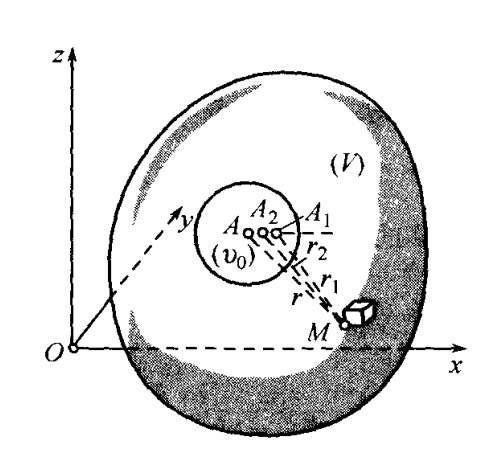
\includegraphics[width=0.5\textwidth]{part3.jpg} % 插入图片,宽度为页面宽度的一半
\end{figure}

从立体 $(V)$ 中取出中心在 $\Delta$ 半径为 $2|h|$ 的球 $(v_0)$(见图),则 $\Delta$ 可表作四项和的形式:
\[
\Delta = \frac{1}{h} \iiint_{(V)} \frac{\rho dv}{r_1} - \frac{1}{h} \iiint_{(v_0)} \frac{\rho dv}{r} + \iiint_{(V)} \rho \left( \frac{1}{h} \left( \frac{1}{r_1} - \frac{1}{r} \right) - \frac{x - \xi}{r^3} \right) dv.
\]

第二及第三项立刻可用当 $r_0 = 2|h|$ 时的不等式 (3-5) 及 (3-6) 来估计:
\[
\frac{1}{|h|} \iiint_{(v_0)} \frac{\rho dv}{r} \leq \frac{2\pi L (2h)^2}{|h|} = 8\pi L |h|,
\]
\[
\iiint_{(v_0)} \frac{\rho(x - \xi)}{r^3} \leq 2\pi L \cdot 2|h| = 4\pi L |h|.
\]

为了方便地估计第一项,绕点 $A_1$ 作一半径为 $3|h|$ 的球;球 $(v_0)$ 整个含在它里面,则再利用不等式 (3-5) 的不等式时,将有
\[
\frac{1}{|h|} \iiint_{(v_1)} \frac{\rho dv}{r_1} \leq \frac{2\pi L (3h)^2}{|h|} = 18\pi L \cdot |h|.
\]

最后,我们来讨论最后一项。如引进函数
\[
f(\xi, \eta, \zeta) = \frac{1}{r},
\]
则在括号中的式子不是别的,恰为
\[
\frac{f(\xi + h, \eta, \zeta) - f(\xi, \eta, \zeta)}{h} - f'_\xi(\xi, \eta, \zeta),
\]
由泰勒公式可换作
\[
\frac{h}{2} f''_{\xi^2}(\xi + \theta h, \eta, \zeta) \quad (0 < \theta < 1)。
\]
但现在
\[
f''_{\xi^2}(\xi, \eta, \zeta) = \frac{3(x - \xi)^2}{r^5} - \frac{1}{r_2^3};
\]
所以
\[
|f''_{\xi^2}(\xi + \theta h, \eta, \zeta)| \leq \frac{4}{r_2^3}。
\]
其中 $r_2$ 是自点 $M$ 到点 $A_2(\xi + \theta h, \eta, \zeta)$ 的距离 $A_2M$。

由三角形 $AM A_2$(见图)有 $A_2M > AM - AA_2$。但点 $M$ 在半径为 $2|h|$ 的球 $(V_0)$ 的外面,
而 $AA_2$ 显然小于 $|h|$,故 $AA_2 < \frac{1}{2}AM$ 且 $A_2M > \frac{1}{2}AM$,即 $r_2 > \frac{1}{2}r$。
注意到所有这些,我们得如下的估计:

\[
\iiint_{(V) - (V_0)} \left| \rho \left\{ \frac{1}{h} \left( \frac{1}{r_1} - \frac{1}{r} \right) - \frac{x - \xi}{r^3} \right\} \right| \, dV 
\leq 16L |h| \cdot \iiint_{(V) - (V_0)} \frac{dV}{r^3}.
\]

取一中心在 $A$ 的球 $(V_1)$,其半径 $R$ 如此地大使立体 $(V)$ 整个含在它里面。则所得式子也就小于

\[
16L |h| \iiint_{(V_1) - (V_0)} \frac{dV}{r^3} 
= 16L |h| \int_{0}^{2\pi} \int_{0}^{\pi} \int_{2|h|}^R \frac{\sin \varphi}{r} \, dr d\varphi d\theta
= 64\pi L \cdot |h| \big( \ln R - \ln 2|h| \big).
\]

最后,
\[
|\Delta| \leq C_1 |h| + C_2 |h| |\ln 2|h||,
\]
其中 $C_1$ 及 $C_2$ 是不难计算的二常数,由此可见,$\Delta$ 与 $h$ 同时趋近于零,则
\[
\frac{\partial W}{\partial \xi} = F_x.
\]

同样可建立关系式 (3-5) 的另外二式。最后,用类似的观察可证明,即使点 $A$ 属于立体 $(V)$ 时,函数 $\frac{\partial W}{\partial \xi}$, $\frac{\partial W}{\partial \eta}$, $\frac{\partial W}{\partial \zeta}$ 连续。

\subsection{第三部分问题证明}
\subsubsection*{Part 1}
由第 $3.2$ 目可知,球 $B(R)$ 对 $P(x_0, y_0, z_0)$ 的引力为
\[
\mathbf{F} = (F_x, F_y, F_z),
\]
其中
\begin{align*}
F_x = \iiint_{B(R)} G \frac{\mu(x, y, z)(x - x_0)}{r^3} \, dV, \\
F_y = \iiint_{B(R)} G \frac{\mu(x, y, z)(y - y_0)}{r^3} \, dV, \\
F_z = \iiint_{B(R)} G \frac{\mu(x, y, z)(z - z_0)}{r^3} \, dV, \\
r = \sqrt{(x - x_0)^2 + (y - y_0)^2 + (z - z_0)^2}
\end{align*}
在这里,$r$是点 $P$ 到元素(或到我们认为它的质量所集中中的点处)的距离。$G$ 为引力常数。

\subsubsection*{Part 2}
由于牛顿引力势的梯度就是引力, 因此从第3.3目的结果即可导出球体对点
P处的质点的引力,若球体为非均质, 但密度函数只与点到球心的距离有关,即$\rho = \rho(r)$,则球体的对空间任意一点$P$的引力可等效为整个球体质量压缩在球心这一质点对点$P$的引力。\cite{15}\cite{16}

其他情况下,不均匀球体对空间任意一点的引力不能与某单个质点的引力等效。


\newpage
\section{第四部分:等周问题}
\setcounter{section}{4} % 手动设置章节编号为 1
\setcounter{subsection}{0} % 手动设置章节编号为 1
\[
\Gamma: x = x(t), \, y = y(t), \, t \in [0, 2\pi]
\]
满足:$x(t), y(t)$ 处处可导,$x'(t)^2 + y'(t)^2$ 处处大于零,且 $\Gamma$ 的周长等于 $2\pi$。试证明:所有满足上述条件的曲线中,圆周所围成的区域面积最大。
\subsection{等周不等式}
等周问题与等周不等式是一个非常悠久的数学问题,在微分几何学中有着重要的意义\cite{key8},下面我们给出平面等周不等式的严格叙述:

\begin{theorem}
设平面 $C^1$ 简单闭曲线 $\Gamma$ 的长度为 $L$, $\Gamma$ 围成的区域面积为 $A$,则成立
\[
L^2 \geq 4\pi A.
\]

等号成立当且仅当 $\Gamma$ 是圆周。
\end{theorem}
这里使用了拓扑学中非常著名的 Jordan 曲线定理: 平面上的简单闭曲线的补集由两个连通分支组成, 其中一
个分支有界, 另一个分支无界。

\vspace{0.2cm}
\noindent **下面给出一种基于Schimdt的思路的等周不等式微分几何证明方法
\begin{proof}
(等周不等式的证明)

设简单闭曲线 $\Gamma$ 的弧长参数化为 $r(s) = (x(s), y(s))$,$s \in [0, L]$。由于 $r(s)$ 的像是平面中的紧集,所以我们可以选取曲线 $\Gamma$ 上的点 $P_1 = r(s_1)$ 和 $P_2 = r(s_2)$,使得在曲像集中,$P_1$ 的 $x$ 坐标取得最小值,而 $P_2$ 的 $x$ 坐标取得最大值,不妨设 $0 \leq s_1 < s_2 \leq L$。

经过 $P_1$ 和 $P_2$,分别作平行于 $y$ 轴的直线 $L_1$ 和 $L_2$,这时 $\Gamma$ 恰好内切于 $L_1, L_2$ 围成的带状域 $S$。我们作 $S$ 的内切圆周 $C$,使得其圆心落在 $x$ 轴上,不妨设为原点。设该内切圆的半径为 $r > 0$。
\begin{figure}[h!] % 图片环境
    \centering % 图片居中
    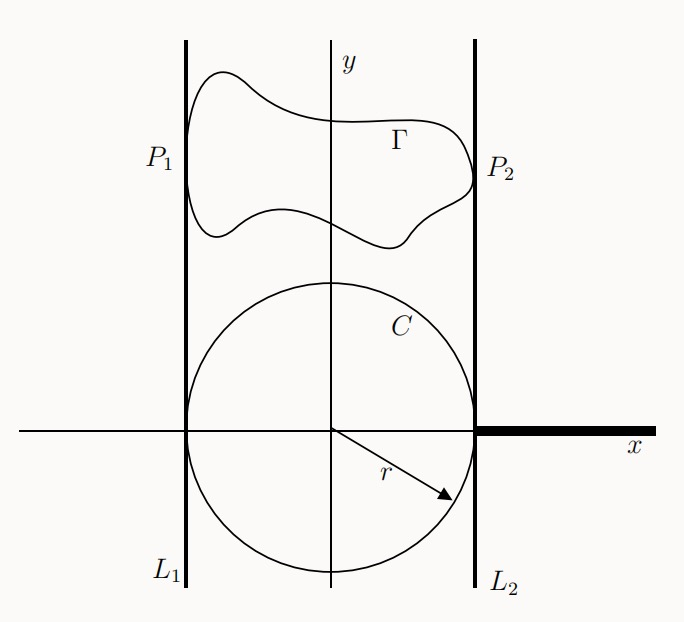
\includegraphics[width=0.5\textwidth]{part4.png} % 插入图片,宽度为页面宽度的一半
\end{figure}

我们给定圆周 $C$ 的一个分段光滑的参数化为 $\tilde{r}(s) = (x(s), z(s))$(注意此时 $s$ 不再为弧长参数)。其中 $z(s)$, $0 \leq s \leq L$ 定义为
\[
z(s) =
\begin{cases} 
    \sqrt{r^2 - x(s)^2}, & s_1 \leq s \leq s_2, \\
    -\sqrt{r^2 - x(s)^2}, & \text{otherwise}.
\end{cases}
\]
根据 Green 公式可得
\[
A = \int_C x \, dy = \int_0^L x(s) y'(s) \, ds, \quad \pi r^2 = \int_C z \, dx = -\int_0^L z(s) x'(s) \, ds.
\]
两式相加,并应用 Cauchy 不等式可得:
\[
A + \pi r^2 = \int_0^L \big( x(s) y'(s) - z(s) x'(s) \big) \, ds
\]
\[
\leq \int_0^L \sqrt{x(s)^2 + z(s)^2} \cdot \sqrt{y'(s)^2 + x'(s)^2} \, ds.
\]
\[
\leq \int_0^L r \cdot 1 \, ds = Lr.
\]
再用一次均值不等式即得:
\[
A = r(L - \pi r) \leq \frac{1}{\pi} \left( \frac{\pi r + L - \pi r}{2} \right)^2 = \frac{L^2}{4\pi}.
\]
等号不等式即证。

下面我们讨论取等条件。如果等号成立,首先从均值不等式的取等条件可得 $r = \frac{L}{2\pi}$。其次,从 Cauchy 不等式的取等条件可得存在函数 $\lambda(s)$,使得
\[
(x(s), -z(s)) = \lambda(s) (y'(s), x'(s)).
\]
由此计算可得
\[
|\lambda(s)| = \sqrt{\frac{x'^2 + z'^2}{y'^2 + x'^2}} = \frac{L}{2\pi}.
\]
这说明 $\lambda = \frac{L}{2\pi}$ 恒为常数,即 $x = \pm z, y = \pm z$。另一方面,我们也可以将 $\Gamma$ 视为两条平行于 $x$ 轴的直线围成带状域的内切圆切线,对应曲周闭圆周 $C': \tilde{r}(s) = (u(s), v(s))$。然后重复之前的过程可得 $y = \pm z$。\cite{key6}所以此时成立:
\[
x(s)^2 + y(s)^2 = \frac{L^2}{4\pi^2}.
\]
这就说明了 $\Gamma$ 是一个圆周。
\end{proof}

\subsection{第四部分问题证明}
根据题目中的描述,这个曲线 $\Gamma$ 是一条 \textbf{Jordan 曲线},因为它符合以下定义特性:
\begin{enumerate}
    \item \textbf{简单闭曲线}:题目明确说明曲线是“简单闭曲线”,这意味着曲线不自交。
    \item \textbf{可导性}:曲线由参数方程 $x = x(t), y = y(t), t \in [0, 2\pi]$ 描述,且 $x(t), y(t)$ 处处可导,保证曲线是光滑的。
    \item \textbf{非零导数}:题目指出 $x'(t)^2 + y'(t)^2 > 0$,确保曲线没有停滞点。
\end{enumerate}

因此,这条曲线满足 Jordan 曲线的基本性质,是一个平面上的闭合、简单的连续曲线,将平面分成两个不相交的区域:内区域和外区域。

故由第4.1目的等周不等式可知,所有满足题设条件的曲线中,圆周所围成的区域面积最大。

\newpage 
% 修改标题为“参考文献”
\addcontentsline{toc}{section}{参考文献}
\printbibliography % 输出文献列表
\end{document}
\end{comment}